\documentclass{cmslatex}   
%\usepackage{latexsym, amssymb, enumerate, amsmath}
\usepackage{graphicx,amssymb,amsmath,amsfonts,mathrsfs}

 %
\sloppy

\thinmuskip = 0.5\thinmuskip \medmuskip = 0.5\medmuskip
\thickmuskip = 0.5\thickmuskip \arraycolsep = 0.3\arraycolsep

\renewcommand{\theequation}{\arabic{section}.\arabic{equation}}

\def\open#1{\setbox0=\hbox{$#1$}
\baselineskip = 0pt \vbox{\hbox{\hspace*{0.4 \wd0}\tiny 
$\circ$}\hbox{$#1$}} \baselineskip = 10pt\!}

\newcommand{\ph}{\hat{\phi}}
\newcommand{\pt}{\tilde{\phi}} 
\newcommand{\pc}{\check{\phi}}
\newcommand{\gh}{\hat{\gamma}}
\newcommand{\Dh}{\hat{\Delta}}
\newcommand{\dha}{\hat{\delta}}
\newcommand{\qh}{\hat{q}}
\newcommand{\xh}{\hat{x}}
\newcommand{\HM}{\mathcal{H}_{\text{max}}}
\newcommand{\Hm}{\mathcal{H}_{\text{min}}}
\newcommand{\sech}{\rm \hspace{0.7mm}sech}
\newcommand{\I}{\mathrm{i}}
\newcommand{\hh}{\hat{h}}
\newcommand{\mh}{m_r}
\newcommand{\mt}{m_i}
\newcommand{\M}{\mathbf{M}}
\newcommand{\X}{\mathbf{X}}
\newcommand{\T}{\mathbf{T}}
\newcommand{\Hb}{\mathbf{H}}
\newcommand{\K}{\mathbf{K}}
\newcommand{\J}{\mathbf{J}}
\renewcommand{\d}{\text{d}}

\newcommand\bsig{\mbox{\boldmath${\sigma}$}}
\newcommand\beps{\mbox{\boldmath${\epsilon}$}}
\newcommand\bxi{\mbox{\boldmath${\xi}$}}
\newcommand\bmu{\mbox{\boldmath${\mu}$}}
\newcommand\balpha{\mbox{\boldmath${\alpha}$}}
\newcommand\brho{\mbox{\boldmath${\rho}$}}
\newcommand\bDelta{\mbox{\boldmath${\Delta}$}}
\newcommand\bXi{\mbox{\boldmath${\Xi}$}}


\newtheorem{thm}{Theorem}[section]
\newtheorem{prop}[thm]{Proposition}
\newtheorem{lem}[thm]{Lemma}
\newtheorem{cor}[thm]{Corollary}

    %\theoremstyle{definition}

\newtheorem{defn}[thm]{Definition}
\newtheorem{notation}[thm]{Notation}
\newtheorem{example}[thm]{Example}
\newtheorem{conj}[thm]{Conjecture}
\newtheorem{prob}[thm]{Problem}

    %\theoremstyle{remark}

\newtheorem{rem}[thm]{Remark}
    % Use the standard latex environments for theorems, etc. Here is one
          % possible method of declaring them: It numbers all results by the
          % section, and uses a common numbering system for the different
          % environmentts.

\begin{document}

\title{Spectral measure computations \\ for composite materials}
%\thanks{%{Received date / Revised version date}
          % The correct dates will be entered by the CMS editor}}
%}}
          %For each author, make a block with the following four
          %macros:
% \author{full name
% \thanks {address, (email).}
% \and full name \thanks {address, (email).}}
%
\author{N. B. Murphy\thanks {murphy@math.utah.edu}
%
\and E. Cherkaev\thanks {elena@math.utah.edu}
%
\and C. Hohenegger\thanks {choheneg@math.utah.edu}
%
\and K. M. Golden\thanks {golden@math.utah.edu}
}
          %{Put the URL for your home page here if you have one}

          %Use \thanks statements for acknowledgments of grants and
          %support. They will appear below all the authors' addresses, so be
          %specific about which author is thanking whom:

          %\thanks{}

\pagestyle{myheadings} \markboth{Spectral measure computations}{Murphy et. al.}\maketitle


\begin{center}
University of Utah, Department of Mathematics \\ 155 S 1400 E
  RM 233, Salt Lake City, UT 84112-0090, USA
\end{center}

\vspace{3ex}


\begin{abstract}
The analytic continuation method of homogenization theory provides
Stieltjes integral representations for the effective parameters of
composite media. These representations involve the spectral measures of self-adjoint random
operators which depend only on the composite geometry. On finite bond
lattices, these random operators are represented by random matrices
and the spectral measures are given explicitly in terms of their
eigenvalues and eigenvectors. Here we provide the mathematical
foundation for rigorous computation of spectral measures for such
composite media, and develop a numerically efficient projection method
to enable such computations. We also introduce a family of
random bond lattices and directly compute the associated spectral
measures and effective parameters. The computed spectral
measures are in excellent agreement with known theoretical
results. The behavior of the associated effective parameters is consistent with
the symmetries and theoretical predictions of models, and the computed values 
fall within rigorous bounds. Some previous calculations of spectral measures
have relied on finding the boundary values of the imaginary part of the 
effective parameter in the complex plane. Our method
instead relies on direct computation of the eigenvalues and eigenvectors, 
which enables, for example, statistical analysis of the spectral data.   
\end{abstract}

\begin{keywords}
composite materials, random resistor network, percolation,
homogenization, spectral measure, random matrix 
\smallskip

{\bf subject classifications.}
% GENERAL: Conference proceedings and collections of papers:
% Conference proceedings and collections of papers 
00B15,
% Measures, integration, derivative, holomorphy (all involving infinite-
% dimensional spaces): Measures and integration on abstract linear spaces
%46G12,
% OPERATOR THEORY: Special classes of linear operators: Hermitian and
% normal operators (spectral measures, functional calculus, etc.)
47B15,
% NUMERICAL ANALYSIS: Numerical linear algebra: Eigenvalues, eigenvectors
65C60,
% MECHANICS OF DEFORMABLE SOLIDS: Generalities, axiomatics,
% foundations of continuum mechanics of solids:
% Random materials and composite materials 
%74A40,
% MECHANICS OF DEFORMABLE SOLIDS: Generalities, axiomatics,
% foundations of continuum mechanics of solids: Nonsimple materials
%74E30,
% FUNCTIONS OF A COMPLEX VARIABLE: Analytic continuation 
30B40,
% OPTICS, ELECTROMAGNETIC THEORY: General: Composite media; random media
78A48,
% OPTICS, ELECTROMAGNETIC THEORY: Basic methods: Spectral methods
%78M22,
% CLASSICAL THERMODYNAMICS, HEAT TRANSFER: Basic methods: Spectral
% methods
%80M22,
% CLASSICAL THERMODYNAMICS, HEAT TRANSFER: Basic methods: Homogenization
80M40,
% PROBABILITY THEORY AND STOCHASTIC PROCESSES: Special processes:
% Interacting random processes; statistical mechanics type models;
% percolation theory
60K35
\end{keywords}


\section{Introduction}\label{Introduction}
%
Over the years a broad range of mathematical techniques have been
developed that reduce the analysis of complex composite materials,
with rapidly varying structures in space, to solving averaged, or
\emph{homogenized} equations involving an effective parameter.
Homogenization for composite media with rapidly varying coefficients
of thermal conductivity,  
electrical conductivity, electrical permittivity, or magnetic permeability,
for example,
was established by Papanicolaou and Varadhan \cite{Papanicolaou:RF-835}
for the steady state, static case with real parameters \cite{MILTON:2002:TC}. 
This work was extended
by Golden and Papanicolaou \cite{Golden:CMP-473,Golden:JSP-655} to the
quasi-static frequency dependent case with complex
parameters. Analysis of the effective dielectric problem for the fully
frequency dependent case described by the Helmholtz equation is given
in \cite{Simeonova:MMS:1113}.




The analytic continuation method (ACM) of homogenization theory
for \emph{two-component} media in the
quasi-static limit was developed by Bergman \cite{Bergman:PRL-1285},
Milton \cite{Milton:APL-300}, and Golden and Papanicolaou
\cite{Golden:CMP-473},
leading to Stieltjes integral representations for the effective
parameters.  The Golden-Papanicolaou formulation of this
method is based on the spectral theorem
and resolvent formulas involving random self-adjoint operators. This
formulation demonstrated that the measures underlying 
these integral representations are \emph{spectral measures} associated
with the random operators, which depend only on the composite
geometry. These measures contain all the information about the mixture
geometry, and provide a link between microgeometry and
transport. Local geometry is encoded in ``geometric'' resonances in
the measures \cite{Jonckheere_Luck_JPA_1998}, while global
connectivity is encoded by spectral gaps in the measures at the
spectral endpoints
\cite{Murphy:JMP:063506,Jonckheere_Luck_JPA_1998}. A remarkable
feature of the method is that once the spectral measures are found for
a given composite geometry, by the spectral coupling of the governing
equations
\cite{Cherkaev:IP-1203,MILTON:2002:TC,Cherkaev:2004:331,Cherkaev:PBCM:0921},
the effective electrical, magnetic, and thermal transport properties
are \emph{all} completely determined by these measures.


 
The integral representations yield rigorous \emph{forward bounds} on
the effective parameters of composites, given partial information on
the microgeometry
\cite{Bergman:PRL-1285,Milton:APL-300,Golden:CMP-473,Bergman:AP-78,Bruno:PRSLA-353}. One  
can also use the integral representations to obtain inverse bounds, 
where data on the electromagnetic response of a sample, for example,
is used to bound its structural parameters, such as the volume
fractions of the components
\cite{McPhedran:APA:19,McPhedran:MRSP:1990:195,Cherkaev:WRM-437,Cherkaev:IP-1203,Cherkaev:IP-065008,Zhang:JCP-5390,Bonifasi-Lista:PMB-3063,Cherkaev:JBiomech-345,Day:JPCM-99,Golden:JBM:337},
and even the separation of the inclusions in 
matrix particle composites \cite{Orum:PRSLA:2012}. Furthermore, the
spectral measure can be \emph{uniquely} reconstructed
\cite{Cherkaev:IP-1203} when the data is given for a continuous
interval of electromagnetic frequency. This, in turn, can be used to
calculate other effective parameters, such as the viscoelastic modulus
\cite{Cherkaev:JBiomech-345}, effective thermal conductivity
\cite{Cherkaev:2004:331,Cherkaev:PBCM:0921}, and recover the associated structural parameters 
\cite{Cherkaev:IP-1203,Cherkaev:IP-065008,Zhang:JCP-5390,Bonifasi-Lista:PMB-3063,Cherkaev:JBiomech-345,Day:JPCM-99,Golden:JBM:337}. 
For classes of composites which undergo a percolation transition
\cite{Stauffer-92,Torquato:RHM-02}, the integral representations have
been used to obtain detailed information regarding the critical
behavior of the effective parameters in the scaling regime
\cite{Golden:PRL-3935,Murphy:JMP:063506}. The relationship between the
effective parameters and the system energy \cite{Murphy:JMP:063506}
has also led to a physically consistent statistical mechanics model for
two-component dielectric media which is also mathematically tractable
\cite{Murphy_Thermo_Stat_Mech}. 




Despite the many applications which have stemmed from the ACM,
explicit analytical calculations of the effective parameters and
spectral measures have been obtained for only a handful of composite
microstructures. There are various numerical methods which have been
used to compute the effective parameters of two-component
composites. These computations may, in principle, be used to compute
the corresponding spectral measures through the Stieltjes--Perron
inversion theorem. This theorem states that the measure is recovered
as a weak limit of the imaginary part of the effective parameter in
the complex plane.




Highly accurate numerical computations of the effective permittivity
for a class of continuum composites which have sharp corners are
described in \cite{Helsing:NJP:115005}. The computations are based on
a multigrid recursive compressed inverse preconditioning method
\cite{Helsing:2008:8820,Helsing:JCP:1171,Helsing:JCP:7533} developed 
for calculation of the effective conductivity of random
checkerboards. In \cite{Day:JPCM-96} the effective 
conductivity of the 2D random resistor network (RRN) 
was computed using an efficient algorithm that implements $Y$-$\Delta$
transformations of the network. In
\cite{Greengard:1994:379,Cheng:1997:629,Greengard:2006:64} the Fast
Multipole Method was exploited to compute the electrostatic fields and
the effective conductivity for two-component matrix particle
composites.      


In \cite{Helsing:NJP:115005,Day:JPCM-96}, the spectral measures
associated with the composite microstructures of interest were
computed using the Stieltjes--Perron inversion theorem. However, the
presence of delta components or essential singularities in the
measures, for example, makes it difficult to resolve details of the
spectrum using this approach. To help overcome this limitation, here
we develop a mathematical framework which provides a rigorous way to
directly compute the spectral measures and effective parameters for
finite lattice composite microstructures, or discretizations of
continuum composites. In this case, the random operators underlying the
integral representations of the effective parameters are represented
by random matrices, and the spectral measures are determined
explicitly by their eigenvalues and eigenvectors.



As a consequence,
our approach provides a direct connection between the statistical
behavior of spectral data of random matrices and the behavior of the
effective transport processes of composites. This, in turn, has
provided a direct connection between the ACM and random matrix theory,
and has shown that transitions in the connectedness or percolation
properties of composites are reflected in the short and long range
eigenvalue correlations of the underlying random matrices
\cite{Murphy_RMT_of_Composites}. Moreover, this transitional behavior
is captured by a one parameter uniersality class of random marix
ensembles and provides a mechanism for the collapse of gaps in the
spectral measures \cite{Murphy_RMT_of_Composites}, which leads to
critical behavior in the effective transport coefficients of
composites \cite{Murphy:JMP:063506}. This characterization of critical
behavior of transport in composites by the statistical properties of
eigenvalues and eigenvectors of random matrices is a key feature of
the ACM and our computational approach. 

    

\section{Mathematical Methods}\label{sec:Mathematical_Methods} 
% {\it The analytic continuation method (general operator
%   case). Spectral measure decomposition. Geometric resonances and gaps
%   in the spectral measure. Lattice systems (random matrix case) and
%   the direct calculation of the spectral measure. Forward bounds. What
%   new structure we found regarding the spectral measure
%   decomposition.} 
%
We now formulate the effective parameter problem for random
two-phase conductive media in the continuum and lattice
settings. In Section \ref{sec:Continuum_Setting} we review and extend
the ACM for the continuum setting \cite{Golden:CMP-473}, while the
\emph{infinite} 
lattice setting \cite{Bruno:JSP-365,Golden:CMP-467} is reviewed in
Section \ref{sec:Infinite_Lattice_Setting}. The mathematical framework
underlying the infinite lattice case is analogous to that of
the continuum case \cite{Bruno:JSP-365}, and the integral
representations for the effective parameters follow with minor
modifications in the theory. In the \emph{finite} lattice setting, the
integral representations for the effective parameters are analogous to
that of the continuum and infinite lattice cases. However,
significant modifications must be made to the underlying mathematical
framework. A key theoretical contribution of this manuscript is the
formulation of the ACM for the finite lattice case, which is discussed
in Section \ref{sec:Finite_Lattice_Setting}.  


\subsection{Continuum Setting}\label{sec:Continuum_Setting}
%
Consider a random two-phase conductive medium filling all of
$\mathbb{R}^d$, which is determined by the probability space
$(\Omega,P)$. Here, $\Omega$ is the set of all  geometric realizations of our
random medium, which is indexed by the parameter $\omega\in\Omega$ representing
one particular geometric realization, and $P$ is the associated
probability measure. Details regarding the underlying sigma-algebra
are discussed in \cite{Papanicolaou:RF-835}. Let $\bsig(\vec{x},\omega)$
and $\brho(\vec{x},\omega)$, $\vec{x}\in\mathbb{R}^d$, be the local complex
conductivity and resistivity tensors associated with the conductive
medium, which are related by $\bsig=\brho^{-1}$ and have components
$\sigma_{jk}(\vec{x},\omega)$ and $\rho_{jk}(\vec{x},\omega)$, $j,k=1,\ldots,d$, that are
(spatially) stationary random fields. 



A \emph{stationary} random field, $f:\mathbb{R}^d\times\Omega\to\mathbb{R}$, is a
field such that the  
joint distribution of $f(\vec{x}_1,\omega),\ldots,f(\vec{x}_n,\omega)$ and that of
$f(\vec{x}_1+\vec{\xi},\omega),\ldots,f(\vec{x}_n+\vec{\xi},\omega)$ is the same for all
$\vec{\xi}\in\mathbb{R}^d$ and $n\in\mathbb{N}$
\cite{Golden:CMP-473,Papanicolaou:RF-835}.
More specifically, we asume that there is a group of transformations
$\tau_x:\Omega\to\Omega$ and measurable functions $f^{\prime}(\omega)=f(0,\omega)$ on $\Omega$ such that
$f(\vec{x},\omega)=f^\prime(\tau_{-x}\,\omega)$ for all $\vec{x}\in\mathbb{R}^d$ and
$\omega\in\Omega$, with $\tau_x\tau_y=\tau_{x+y}$.  Moreover, we shall assume that the
group is one-to-one and preserves the measure $P$, i.e. $P(\tau_xA)=P(A)$
for all $P$-measurable sets $A$
\cite{Golden:CMP-473,Papanicolaou:RF-835}. For notational simplicity,
we will not distinguish between the functions $f^\prime:\Omega\to\mathbb{R}$ and
$f:\mathbb{R}^d\times\Omega\to\mathbb{R}$, as the context of each notation is now
clear. 






The group of transformations $\tau_x$ acting on $\Omega$ induces a group of
operators $T_x$ on the Hilbert space $L^2(\Omega,P)$ defined by
$(T_xf)(\omega)=f(\tau_{-x}\,\omega)$ for all $f\in L^2(\Omega,P)$. Since $\tau_x$ is measure
preserving, the operators $T_x$ form a unitary group and therefore
have closed densely defined infinitesimal generators $L_i$ in each
direction $i=1,\ldots,d$ with domain $\mathscr{D}_i\subset L^2(\Omega,P)$
\cite{Golden:CMP-473,Papanicolaou:RF-835}. Thus,  
%
\begin{align}\label{eq:Li}
  L_i=\left.\frac{\partial}{\partial x_i}T_x \right|_{x=0}, \quad i=1,\ldots,d,
\end{align}
%
where $x_i$
%$x_i=(\vec{x}_i)$
is the $i^{\,\text{th}}$ component of the vector
$\vec{x}$ and differentiation is defined in the sense of convergence
in $L^2(\Omega,P)$ for elements of $\mathscr{D}_i$
\cite{Golden:CMP-473}. The closed subset
$\mathscr{D}=\cap_{i=1}^d\mathscr{D}_i$ of $L^2(\Omega,P)$ is a Hilbert space
\cite{Golden:CMP-473} with inner product $\langle \cdot,\cdot\rangle_D$ given by  $\langle
f,g\rangle_D=\langle f,g\rangle_{L^2}+\sum_{i=1}^d\langle L_if,L_ig\rangle_{L^2}$, where $\langle\cdot,\cdot\rangle_{L^2}$
is the $L^2(\Omega,P)$ inner product. 



Consider the Hilbert space $\mathscr{H}=\bigotimes_{i=1}^dL^2(\Omega,P)$ with inner
product $\langle\cdot,\cdot\rangle$ defined by $\langle\vec{\xi},\vec{\zeta}\rangle=\langle\vec{\xi}\cdot\vec{\zeta}\rangle$, where
$\vec{\xi}\cdot\vec{\zeta}=\vec{\xi}^{\;\,T}\vec{\zeta}$ denotes the dot-product 
on $\mathbb{R}^d$ and $\langle\cdot\rangle$ means ensemble average over $\Omega$ or, by an
ergodic theorem \cite{Golden:CMP-473}, spatial average over all of
${\mathbb{R}}^d$. Define the Hilbert spaces \cite{Golden:CMP-473} of
``curl free'' $\mathscr{H}_\times$ and ``divergence free''
$\mathscr{H}_{\bullet}$ random fields  
%
\begin{align}\label{eq:curlfreeHilbert}
  &\mathscr{H}_\times=
  \left\{\vec{Y}\in \mathscr{H} \ | \ \vec{\nabla} \times\vec{Y}=0 \text{ weakly and }
    \langle\vec{Y}\rangle=0
  \right\}, \\
&\mathscr{H}_{\bullet}=
\left\{\vec{Y}\in \mathscr{H} \ | \ \vec{\nabla}\cdot\vec{Y}=0 \text{ weakly and }
    \langle\vec{Y}\rangle=0\right\},\notag 
\end{align}  
%
% \begin{align}\label{eq:curlfreeHilbert_Precise}
%   &\mathscr{H}_\times=
%   \left\{Y_i(\omega)\in L^2(\Omega,P), \ i=1,\ldots,d \ | \ L_iY_j-L_jY_i=0 \text{ weakly and }
%     \langle Y_i\rangle=0\right\},
%     \\
%   &\mathscr{H}_\bullet=
%   \left\{Y_i(\omega)\in L^2(\Omega,P), \ i=1,\ldots,d \ \Big| \ \sum_{i=1}^dL_iY_i=0 \text{ weakly and }
%     \langle Y_i\rangle=0\right\}.
%     \notag
% \end{align}
% %
% where $j=1,\ldots,d$.
%
where we have used the simplified notation $\langle\vec{Y}\rangle=0 \iff \langle Y_i\rangle=0$ for
all $i=1,\ldots,d$, $\vec{\nabla}\cdot\vec{Y}=\sum_{i=1}^dL_iY_i$, and $\vec{\nabla} \times\vec{Y}=0$
means $L_iY_j-L_jY_i=0$ for all $i,j=1,\ldots,d$. Consider the following
variational problems \cite{Golden:CMP-473}. Find
$\vec{E}_f\in\mathscr{H}_\times$ and $\vec{J}_f\in\mathscr{H}_\bullet$ such that     
%
\begin{align}
 \label{eq:Weak_Curl_Free_Variational_Form}
 &\langle\bsig(\vec{E}_0+\vec{E}_f)\cdot\vec{Y}\rangle=0 \quad  \forall \
  \vec{Y}\in\mathscr{H}_\times &&\text{and}
%
 &&\langle\brho(\vec{J}_0+\vec{J}_f)\cdot\vec{Y}\rangle=0 \quad  \forall \
  \vec{Y}\in\mathscr{H}_{\bullet}\,,  
\end{align}
%
respectively. When the bilinear forms
$\Psi(\vec{\xi},\vec{\zeta})=\bsig\,\vec{\xi}\cdot\vec{\zeta}\;$ and
$\Phi(\vec{\xi},\vec{\zeta})=\brho\,\vec{\xi}\cdot\vec{\zeta}\;$ are bounded and
coercive, these problems have unique solutions
\cite{Golden:CMP-473,Papanicolaou:RF-835} satisfying the quasi-static
limit of Maxwell's equations  \cite{Jackson-1999} 
%
\begin{align}   \label{eq:Maxwells_Equations_E}  
 &\vec{\nabla}\times\vec{E}=0, \quad
  \vec{\nabla}\cdot\vec{J}=0,\quad
  \vec{J}=\bsig\vec{E},\quad
  %\vec{E}=\vec{E}_0+\vec{E}_f, \quad
  \langle\vec{E}\,\rangle=\vec{E}_0, \\
%
  %\label{eq:Maxwells_Equations_D}
   &\vec{\nabla}\times\vec{E}=0, \quad
   \vec{\nabla}\cdot\vec{J}=0, \quad
   \vec{E}=\brho\vec{J},\quad
   %\vec{J}=\vec{J}_0+\vec{J}_f,\quad
   \langle\vec{J}\,\rangle=\vec{J}_0.
   \notag  
\end{align}
%
Here, $\vec{E}(\vec{x},\omega)=\vec{E}_0+\vec{E}_f(\vec{x},\omega)$ is the
random electric field, where $\vec{E}_f$ is the fluctuating field of
mean zero about the (constant) average $\vec{E}_0$. Similarly,
$\vec{J}(\vec{x},\omega)=\vec{J}_0+\vec{J}_f(\vec{x},\omega)$ is the random  
current density. Moreover, $\vec{E}_f$ and $\vec{J}_f$ are stationary
random fields \cite{Golden:CMP-473}. 
% In component form equation \eqref{eq:Maxwells_Equations_E} is given by
% %
% \begin{align}   \label{eq:Maxwells_Equations_Component}  
%   \partial_{x_j}E_i-\partial_{x_i}E_j=0, \quad
%   \sum_{j=1}^d\partial_{x_j}D_j=0, \quad
%   D_j=\sum_{k=1}^d\sigma_{jk}E_k, \quad
% %  \vec{E}=\vec{E}_0+\vec{E}_f, \quad
%   \langle\vec{E}\,\rangle=\vec{E}_0, 
% \end{align}




As $\vec{E}_f\in\mathscr{H}_\times$ and $\vec{J}_f\in\mathscr{H}_\bullet$, equation
\eqref{eq:Weak_Curl_Free_Variational_Form} yields the energy (power)
\cite{Jackson-1999} constraints $\langle\vec{J}\cdot\vec{E}_f\rangle=0$ and
$\langle\vec{E}\cdot\vec{J}_f\rangle=0$, respectively, which leads to the following
reduced energy representations $\langle\vec{J}\cdot\vec{E}\rangle=\langle\vec{J}\rangle\cdot\vec{E}_0$
and $\langle\vec{E}\cdot\vec{J}\rangle=\langle\vec{E}\rangle\cdot\vec{J}_0$. The effective complex
conductivity and resistivity tensors, $\bsig^*$ and $\brho^*$, are
defined by   
%
\begin{align}\label{eq:eff_eps_def}
    \langle \vec{J} \,\rangle=  \bsig^* \vec{E}_0
    \quad \text{and} \quad    
    \langle \vec{E} \,\rangle=  \brho^*\vec{J}_0.
\end{align}
%
Consequently, we have the following energy representations involving
the effective parameters 
%$\langle\vec{J}\cdot\vec{E}\rangle=\bsig^*\vec{E}_0\cdot\vec{E}_0=\brho^*\vec{J}_0\cdot\vec{J}_0$.
%
\begin{align}\label{eq:Energy_Reps}
  \langle\vec{J}\cdot\vec{E}\rangle=\bsig^*\vec{E}_0\cdot\vec{E}_0=\brho^*\vec{J}_0\cdot\vec{J}_0
\end{align}
%


We assume that the composite is a locally isotropic random medium so
that $\sigma_{jk}(\vec{x},\omega)=\sigma(\vec{x},\omega)\delta_{jk}$ and
$\rho_{jk}(\vec{x},\omega)=\rho(\vec{x},\omega)\delta_{jk}$, where $\delta_{jk}$ is the
Kronecker delta and $j,k=1,\ldots,d$. We further assume that the composite
is a two-component medium, so that $\sigma(\vec{x},\omega)$ takes the
\emph{complex} values $\sigma_1$ and $\sigma_2$, and $\rho(\vec{x},\omega)$ takes the
complex values $1/\sigma_1$ and $1/\sigma_2$, and satisfy \cite{Golden:CMP-473}
% 
\begin{align}\label{eq:two-phase_eps}
  \sigma(\vec{x},\omega)=\sigma_1\chi_1(\vec{x},\omega)+\sigma_2\chi_2(\vec{x},\omega), \qquad
  \rho(\vec{x},\omega)=\chi_1(\vec{x},\omega)/\sigma_1+\chi_2(\vec{x},\omega)/\sigma_2.
\end{align}
%
%$\sigma(\vec{x},\omega)=\sigma_1\chi_1(\vec{x},\omega)+\sigma_2\chi_2(\vec{x},\omega)$,
Here, $\chi_i(\vec{x},\omega)$ is the characteristic function of medium
$i=1,2$, which equals one for all $\omega\in\Omega$ having medium $i$ at $\vec{x}$
and zero otherwise, with $\chi_1=1-\chi_2$. For simplicity, we focus on one
component, $\sigma^*_{jk}=(\bsig^*)_{jk}$ and $\rho^*_{jk}=(\brho^*)_{jk}$, of
these symmetric tensors, for some $j,k=1,\ldots,d$.  



Due to the homogeneity of these functions,
e.g. $\sigma_{jk}^*(a\sigma_1,a\sigma_2)=a\sigma_{jk}^*(\sigma_1,\sigma_2)$ for any complex number
$a$, they depend only on the ratio $h=\sigma_1/\sigma_2$, and we define the
tensor-valued functions $\mathbf{m}(h)=\bsig^*/\sigma_2$,
$\mathbf{w}(z)=\bsig^*/\sigma_1$, $\tilde{\mathbf{m}}(h)=\sigma_1\brho^*$, and
$\tilde{\mathbf{w}}(z)=\sigma_2\brho^*$ with components  
%
\begin{align}\label{eq:m_h}
  m_{jk}(h)=\sigma_{jk}^*/\sigma_2, \quad
  w_{jk}(z)=\sigma_{jk}^*/\sigma_1, \quad
   \tilde{m}_{jk}(h)=\sigma_1\rho_{jk}^*, \quad
   \tilde{w}_{jk}(z)=\sigma_2\rho_{jk}^*.
\end{align}
%
where $z=1/h$. The dimensionless functions $m_{jk}(h)$ and
$\tilde{m}_{jk}(h)$ are analytic off the negative real axis in the
$h$-plane, while $w_{jk}(z)$ and $\tilde{w}_{jk}(z)$ are analytic off
the negative real axis in the $z$-plane \cite{Golden:CMP-473}. Each
take the corresponding upper half plane to the upper half plane and
are therefore examples of Herglotz functions
\cite{Deift:2000:RMT,Golden:CMP-473}.



A key step in the ACM is
obtaining Stieltjes integral representations for $\bsig^*$ and
$\brho^*$. These follow from resolvent representations for the
electric field $\vec{E}$ \cite{Golden:CMP-473} and current density
$\vec{J}$ \cite{Murphy:JMP:063506}         
%
\begin{align}\label{eq:Resolvent_representations_E_D}
  &\vec{E}=s(sI-\Gamma\chi_1)^{-1}\vec{E}_0=t(tI-\Gamma\chi_2)^{-1}\vec{E}_0 ,
  \quad
   s\in\mathbb{C}\backslash[0,1],\\
  &\vec{J}=t(tI-\Upsilon\chi_1)^{-1}\vec{J}_0=s(sI-\Upsilon\chi_2)^{-1}\vec{J}_0 ,
  \quad
   t\in\mathbb{C}\backslash[0,1].\notag 
\end{align}
%
where $I$ is the identity operator on $\mathbb{R}^d$ and we have
defined the complex variables $s=1/(1-h)$ and $t=1/(1-z)=1-s$. 
The operator $\Gamma=\vec{\nabla}(\Delta^{-1})\vec{\nabla}\cdot$ is based on
convolution with the free-space Green's function for the Laplacian
$\Delta=\vec{\nabla}\cdot\vec{\nabla}=\nabla^{\,2}$, and the operator
$\Upsilon=\vec{\nabla}\times(\vec{\nabla}\times\vec{\nabla}\times)^{-1}\vec{\nabla}\times$ involves the vector
Laplacian $\bDelta=- \vec{\nabla}\times\vec{\nabla}\times + \vec{\nabla}\vec{\nabla}\cdot $ when $d=3$
\cite{Golden:CMP-473,Murphy:JMP:063506}. These (non-random)
integro-differential operators are discussed in more detail below.      



If the current density $\vec{J}(\vec{x},\omega)$ and the electric
field $\vec{E}(\vec{x},\omega)$ are sufficiently smooth for all
$\vec{x}\in\mathbb{R}^d$ when $\omega\in\Omega$, equation 
\eqref{eq:Resolvent_representations_E_D} is obtained as
follows. The operator $\Delta^{-1}$ is
well defined in terms of convolution with respect to the free-space
Green's function of the Laplacian $\Delta$
\cite{Golden:CMP-473,Folland:95}. Similarly, the inverse
$\bDelta^{-1}$ of the vector Laplacian $\bDelta$ is defined in terms
of component-wise convolution with respect to the free-space Green's
function of the Laplacian.

 

Applying the
%integro-differential
operator $\vec{\nabla}(\Delta^{-1})$ to the
formula $\vec{\nabla}\cdot\vec{J}=0$ in equation
\eqref{eq:Maxwells_Equations_E} yields $\Gamma\vec{J}=0$, where
$\Gamma=\vec{\nabla}(\Delta^{-1})\vec{\nabla}\cdot$ is an orthogonal projection
\cite{Golden:CMP-473} from $\mathscr{H}$ onto the Hilbert space
$\mathscr{H}_\times$ of curl-free random fields,
$\Gamma:\mathscr{H}\mapsto\mathscr{H}_\times$. More specifically, for every
sufficiently smooth $\vec{\zeta}\in\mathscr{H}_\times$ there exists
\cite{Jackson-1999} a scalar potential $\varphi$ which is unique up to a 
constant such that $\vec{\zeta}=\vec{\nabla}\varphi$. Consequently, it is clear
that $\Gamma\vec{\zeta}=\vec{\zeta}$ for all such $\vec{\zeta}\in\mathscr{H}_\times$. 


In order to discuss analogous properties of divergence free vector
fields, for simplicity, we restrict our attention to $d=2,3$,
%and avoid a more involved discussion regarding differential forms
%\cite{Darling:Differential_Forms:1994}.
Applying the integro-differential
operator $\vec{\nabla}\times(\bDelta^{-1})$ to the formula
$\vec{\nabla}\times\vec{E}=0$ in equation \eqref{eq:Maxwells_Equations_E} yields  
$\Upsilon\vec{E}=0$, where $\Upsilon=-\vec{\nabla}\times(\bDelta^{-1})\vec{\nabla}\times$ is an
orthogonal projection from $\mathscr{H}$ onto the Hilbert space 
$\mathscr{H}_{\bullet}$ of divergence-free random fields (of transverse
gauge) \cite{Murphy:JMP:063506}. This can be seen as  
follows. For every sufficiently smooth $\vec{\zeta}\in\mathscr{H}_\bullet$ we have
the representation
$\vec{\zeta}=\vec{\nabla}\times(\vec{A}+\vec{C})$, where $\vec{A}$ is a vector
potential associated with $\vec{\zeta}$ and the arbitrary vector field
$\vec{C}$ satisfies $\vec{\nabla}\times\vec{C}=0$ \cite{Jackson-1999}. Without
loss of generality, $\vec{C}$ can be chosen so that $\vec{A}$
satisfies $\vec{\nabla}\cdot\vec{A}=0$ \cite{Jackson-1999}. Hence,
$\vec{\nabla}\times\vec{\zeta}=\vec{\nabla}\times\vec{\nabla}\times\vec{A}
=\vec{\nabla}(\vec{\nabla}\cdot\vec{A})-\bDelta\vec{A}=-\bDelta\vec{A}$. The vector 
$\vec{C}$ chosen in this manner gives the transverse \emph{gauge} of
$\vec{\zeta}$ \cite{Jackson-1999}. Choosing the members of 
$\mathscr{H}_\bullet$ to have transverse gauge, the action of
$\vec{\nabla}\times\vec{\nabla}\times$ on $\mathscr{H}_\bullet$ is given by that of
$-\bDelta$. Therefore, the action of $\Upsilon$ on $\mathscr{H}_\bullet$ is given
by that of 
%$\Upsilon=\vec{\nabla}\times(\vec{\nabla}\times\vec{\nabla}\times)^{-1}\vec{\nabla}\times=\vec{\nabla}\times(\bDelta^{-1})\vec{\nabla}\times$, 
%
\begin{align}\label{eq:GammaCurl}
  \Upsilon=\vec{\nabla}\times(\vec{\nabla}\times\vec{\nabla}\times)^{-1}\vec{\nabla}\times
  =-\vec{\nabla}\times(\bDelta^{-1})\vec{\nabla}\times, 
\end{align}
%
and it is clear from the above discussion that $\Upsilon\vec{\zeta}=\vec{\zeta}$ for
all such $\vec{\zeta}\in\mathscr{H}_\bullet$.
%Unresolved Issue:IS THIS TRUE NOW THAT WE ARE DEALING WITH THE $L_i$
%AS DIFFERENTIAL OPERATORS?





We now derive the formulas in equation
\eqref{eq:Resolvent_representations_E_D}.
Write $\sigma$ and $\rho$ in 
equation \eqref{eq:two-phase_eps} as $\sigma=\sigma_2(1-\chi_1/s)=\sigma_1(1-\chi_2/t)$ and
$\rho=(1-\chi_2/s)/\sigma_1=(1-\chi_1/t)/\sigma_2$. Recall that
$\vec{E}=\vec{E}_0+\vec{E}_f$, where $\vec{E}_0$ is a \emph{constant}
field and $\vec{E}_f\in\mathscr{H}_\times$ so that
$\Gamma\vec{E}=\vec{E}_f$, and similarly
$\Upsilon\vec{J}=\vec{J}_f$. Consequently, from $\Gamma\vec{J}=0$ and $\Upsilon\vec{E}=0$
we have the following formulas which are equivalent to that in 
\eqref{eq:Resolvent_representations_E_D}  
% 
\begin{align}\label{eq:Proj_rep_Ef_Jf}
  \vec{E}_f=\frac{1}{s}\Gamma\chi_1\vec{E}=\frac{1}{t}\Gamma\chi_2\vec{E}, \qquad
  \vec{J}_f=\frac{1}{t}\Upsilon\chi_1\vec{J}=\frac{1}{s}\Upsilon\chi_2\vec{J}.
\end{align}
%
In general, the differential opperators $\vec{\nabla}$, $\vec{\nabla}\cdot$, and
$\vec{\nabla}\times$ are interpreted
in a weak sense in terms of the operators $L_i$ in \eqref{eq:Li}
\cite{Golden:CMP-473}. 



On the Hilbert space $\mathscr{H}_\times$, the operators $\Gamma$ and $\chi_i$,
$i=1,2$, act as projectors \cite{Golden:CMP-473}. Therefore 
$M_i=\chi_i\Gamma\chi_i$, $i=1,2$, are compositions of projection operators on
$\mathscr{H}_\times$, and are consequently positive definite and bounded by
1 in the underlying operator norm \cite{Rudin:87}. They are
self-adjoint with respect to the $\mathscr{H}$-inner-product $\langle\cdot,\cdot\rangle$
\cite{Golden:CMP-473}. Therefore, on the Hilbert space $\mathscr{H}_\times$
with weight $\chi_1$ in the inner-product, $\langle\cdot,\cdot\rangle_1=\langle\chi_1\,\cdot,\cdot\rangle$ for
example, $\Gamma\chi_1$ is a bounded linear self-adjoint operator with
spectrum contained in the interval $[0,1]$
\cite{Golden:CMP-473,Folland:95,Rudin:87}. Hence the resolvent
operator $(sI-\Gamma\chi_1)^{-1}$ in \eqref{eq:Resolvent_representations_E_D}
is also a linear self-adjoint operator with respect to the same
inner-product, and is bounded for  $s\in\mathbb{C}\backslash[0,1]$
\cite{Stone:64}. Similarly, $(tI-\Upsilon\chi_1)^{-1}$ in
\eqref{eq:Resolvent_representations_E_D} is a linear self-adjoint
operator on $\mathscr{H}_\bullet$ with respect to the inner-product
$\langle\cdot,\cdot\rangle_1$, and is bounded for $t\in\mathbb{C}\backslash[0,1]$.





To obtain integral representations for $\bsig^*$ and
$\brho^*$, it is more convenient to consider the functions 
$F_{jk}(s)=\delta_{jk}-m_{jk}(h)$ and $E_{jk}(s)=\delta_{jk}-\tilde{m}_{jk}(h)$
which are analytic off $[0,1]$ in the $s$-plane, and
$G_{jk}(t)=\delta_{jk}-w_{jk}(z)$ and $H_{jk}(t)=\delta_{jk}-\tilde{w}_{jk}(z)$
which are analytic off $[0,1]$ in the $t$-plane
\cite{Golden:CMP-473}. For the formulation of the effective parameter
problem involving $\mathscr{H}_\times$ and $\bsig^*$, define the
coordinate system so that in \eqref{eq:eff_eps_def} the constant
vector $\vec{E}_0$ is given by $\vec{E}_0=E_0\,\vec{e}_j$, where
$\vec{e}_j$ is the standard basis vector on $\mathbb{R}^d$ in the
$j^{\,\text{th}}$ direction for some $j=1,\ldots,d$. In the other
formulation involving $\mathscr{H}_\bullet$ and $\brho^*$, define
$\vec{J}_0=J_0\,\vec{e}_j$. Equations \eqref{eq:eff_eps_def} and 
\eqref{eq:Resolvent_representations_E_D}, and the spectral theorem for
bounded linear self-adjoint operators \cite{Reed-1980,Stone:64} then
yield the following integral representations
\cite{Golden:CMP-473,Bergman:PRC-377,Bergman:AP-78,Murphy:JMP:063506}  
for the effective parameters $\sigma^*_{jk}$ and $\rho^*_{jk}$ (see Section
\ref{sec:The_Spectral_Theorem_Continuum} for details)
%
\begin{align}\label{eq:Stieltjes_F}
  &m_{jk}(h)=\delta_{jk}-F_{jk}(s), \qquad
  F_{jk}(s)=\langle\chi_1(sI-\Gamma\chi_1)^{-1}\vec{e}_j\cdot\vec{e}_k\rangle=\int_0^1\frac{\d\mu_{jk}(\lambda)}{s-\lambda}\,,
  \\
  &w_{jk}(z)=\delta_{jk}-G_{jk}(t), \qquad
  G_{jk}(t)=\langle\chi_2(tI-\Gamma\chi_2)^{-1}\vec{e}_j\cdot\vec{e}_k\rangle=\int_0^1\frac{\d\alpha_{jk}(\lambda)}{t-\lambda}\,,
  \notag \\
  &\tilde{m}_{jk}(h)=\delta_{jk}-E_{jk}(s), \qquad
  E_{jk}(s)=\langle\chi_2(sI-\Upsilon\chi_2)^{-1}\vec{e}_j\cdot\vec{e}_k\rangle=\int_0^1\frac{\d\eta_{jk}(\lambda)}{s-\lambda}\,,
  \notag \\
  &\tilde{w}_{jk}(z)=\delta_{jk}-H_{jk}(t), \qquad
  H_{jk}(t)=\langle\chi_1(tI-\Upsilon\chi_1)^{-1}\vec{e}_j\cdot\vec{e}_k\rangle=\int_0^1\frac{\d\kappa_{jk}(\lambda)}{t-\lambda}\,.
  \notag
\end{align}
%
Here, $\d\mu_{jk}$ and $\d\alpha_{jk}$ are \emph{spectral measures} associated
with the random operators $\chi_1\Gamma\chi_1$ and $\chi_2\Gamma\chi_2$, respectively, while
$\d\eta_{jk}$ and $\d\kappa_{jk}$ are spectral measures associated
with the random operators $\chi_2\Upsilon\chi_2$ and $\chi_1\Upsilon\chi_1$, respectively. More
specifically, there is a one-to-one correspondence between the bounded
linear operator $\chi_1\Gamma\chi_1$ on $\mathscr{H}_\times$, for example, and a
family of projection operators $Q(\lambda)$ parameterized by $\lambda\in[0,1]$ which
satisfies $\lim_{\lambda\to0}Q(\lambda)=0$ and $\lim_{\lambda\to1}Q(\lambda)=I$, where $0$ and $I$
are the null and identity operators on $\mathscr{H}_\times$, respectively
\cite{Stone:64}. The function $\mu_{jk}(\lambda)=\langle Q(\lambda)\vec{e}_j,\vec{e}_k\rangle_1$
is strictly increasing and of bounded variation \cite{Stone:64}.
The spectral measure $\d\mu_{jk}(\lambda)$ is a \emph{Stieltjes measure}
\cite{Folland:99} associated with the function $\mu_{jk}(\lambda)$
\cite{Stone:64} (see Section \ref{sec:The_Spectral_Theorem_Continuum}
for more details). For notational simplicity, we will often refer to
the measure $\mu_{jk}$, not to be confused with the function $\mu_{jk}(\lambda)$. 


By the Stieltjes--Perron inversion theorem
\cite{Henrici:1974:v2,MILTON:2002:TC}, the matrix valued function
$\bmu(\lambda)$ with components $\mu_{jk}(\lambda)$, $j,k=1,\ldots,d$, for example, is
given by the weak limit  
$\bmu(\lambda)=-(1/\pi)\lim_{\varepsilon\downarrow0}\text{Im}(\mathbf{F}(\lambda+\I\varepsilon))$, i.e., 
%
\begin{align}\label{eq:weak_limit_mu}
  \int_0^1\xi(\lambda)\;\d\bmu(\lambda)
  =-\frac{1}{\pi}\lim_{\varepsilon\downarrow0}
        \int_0^1\xi(\lambda)\;\text{Im}(\mathbf{F}(\lambda+\I\varepsilon))\, \d\lambda,
\end{align}
%
for all smooth test functions $\xi(\lambda)$, where
$[\mathbf{F}(s)]_{jk}=F_{jk}(s)$ and
$[\d\bmu(\lambda)]_{jk}=\d\mu_{jk}(\lambda)$. From equation 
\eqref{eq:weak_limit_mu} and the identities 
$m_{jk}(h)=h\,w_{jk}(z)$ and $\tilde{m}_{jk}(h)=h\,\tilde{w}_{jk}(z)$,
which follow from equation \eqref{eq:m_h}, it can be
shown \cite{Murphy:JMP:063506} that the functions $\mu_{jk}(\lambda)$ and
$\alpha_{jk}(\lambda)$, and the functions $\eta_{jk}(\lambda)$ and $\kappa_{jk}(\lambda)$ are
related by
%
\begin{align}\label{eq:Measure_Relations}
  &\lambda\alpha_{jk}(\lambda)=(1-\lambda)\mu_{jk}(1-\lambda)+\lambda\varrho(\lambda), \qquad
  \d\varrho(\lambda)=m_{jk}(0)\delta_0(\d\lambda)+w_{jk}(0)(\lambda-1)\delta_1(\d\lambda),
  \notag     \\
  &\lambda\kappa_{jk}(\lambda)=(1-\lambda)\eta_{jk}(1-\lambda)+\lambda\tilde{\varrho}(\lambda), \qquad
  \d\tilde{\varrho}(\lambda)=\tilde{m}_{jk}(0)\delta_0(\d\lambda)+\tilde{w}_{jk}(0)(\lambda-1)\delta_1(\d\lambda).  
\end{align}
%
% %
% \begin{align}%\label{eq:Measure_Relations}
%   &\lambda\alpha_{jk}(\lambda)=(1-\lambda)\mu_{jk}(1-\lambda)+ 
%        \lambda\,(\,m_{jk}(0)\delta_0(\lambda)+w_{jk}(0)(\lambda-1)\delta_1(\lambda)\,),
%   \\
%   &\lambda\kappa_{jk}(\lambda)=(1-\lambda)\eta_{jk}(1-\lambda) +
%        \lambda\,(\,\tilde{m}_{jk}(0)\delta_0(\lambda)+\tilde{w}_{jk}(0)(\lambda-1)\delta_1(\lambda)\,).
%   \notag     
% \end{align}
% %
Here, $m(0)=m(h)|_{h=0}$ and $w(0)=w(z)|_{z=0}$, for example, and
$\delta_a(\d\lambda)$ is the delta measure concentrated at $\lambda=a$. Equations
\eqref{eq:Stieltjes_F} and \eqref{eq:Measure_Relations} demonstrate
the many symmetries between 
the functions $m_{jk}(h)$, $w_{jk}(z)$, $\tilde{m}_{jk}(h)$, and
$\tilde{w}_{jk}(z)$, and the respective measures $\mu_{jk}$, $\alpha_{jk}$,
$\eta_{ij}$, and $\kappa_{jk}$. Because of these symmetries, for simplicity,
we will focus on $m_{jk}(h)$ and $\mu_{jk}$, and will reintroduce the
other functions and measures where appropriate.  



A key feature of equations \eqref{eq:eff_eps_def}, \eqref{eq:m_h}, and
\eqref{eq:Stieltjes_F} is that the parameter information in $h$ and
$E_0$ is \emph{separated} from the geometry of the composite, which is
encoded in the spectral measure $\mu_{jk}$ via its moments $\mu_{jk}^n$
\cite{Golden:CMP-473,Bruno:JSP-365}
%$\mu_{jk}^n=\int_0^1\lambda^n\d\mu_{jk}(\lambda)$, $n=0,1,2,\ldots$.
%
\begin{align}\label{eq:Moments_mu}
  \mu_{jk}^n=\int_0^1\lambda^n\d\mu_{jk}(\lambda)       
       %=\langle[\Gamma \chi_1]^n\,\vec{e}_j\cdot\vec{e}_k\rangle_1,
       =\langle\chi_1[\Gamma \chi_1]^n\,\vec{e}_j\cdot\vec{e}_k\rangle,
  \quad n=0,1,2,\ldots.,
\end{align}
%
where the second equality follows from the spectral theorem displayed
in equation \eqref{eq:Spectral_Theorem} with $f(\lambda)=\lambda^n$. Since $\chi_1$
operates pointwise on $\mathbb{R}^d$ and the constant vectors
$\vec{e}_j$, $j=1,\ldots,d$, are non-random, we see from equation
\eqref{eq:Moments_mu} that the mass $\mu_{jk}^0$ of the measure
$\mu_{jk}$ is given by
%$\mu_{jk}^0=p_1\delta_{jk}$,
%
\begin{align}
  \mu_{jk}^0=p_1\delta_{jk},
\end{align}
%
where $p_1=\langle\chi_1\rangle$ is the volume fraction of material component
one. This demonstrates that the diagonal components $\mu_{kk}$,
$k=1,\ldots,d$, of $\bmu$ are \emph{positive measures}, 
while the off-diagonal components $\mu_{jk}$, $j\neq k$, have 
zero mass and are consequently \emph{signed measures}
\cite{Folland:99,Rudin:87}. The positivity of the measure $\mu_{kk}$ also
follows from the fact that $Q(\lambda)$ is a \emph{self-adjoint projector}
on $\mathscr{H}_\times$ and $\|Q(\lambda)\vec{e}_k\|_1^2$ is a strictly increasing
function of $\lambda$ \cite{Reed-1980,Stone:64}. Therefore, the measure of
an arbitrary set $A\subseteq[0,1]$ is positive:
% 
\begin{align}\label{eq:Mass_Sign_Measures}   
   &\mu_{kk}(A)=\int_Ad\mu_{kk}=\int_Ad\langle Q(\lambda)\vec{e}_k\cdot\vec{e}_k\rangle_1
       =\int_Ad\langle Q(\lambda)\vec{e}_k\cdot Q(\lambda)\vec{e}_k\rangle_1
       =\int_Ad\|Q(\lambda)\vec{e}_k\|_1^2\geq0,
\end{align}
%
where $\|\cdot\|_1$ denotes the norm induced by the inner-product
$\langle\cdot,\cdot\rangle_1$. 



The higher order moments $\mu_{jk}^n$, $n=1,2,3,\ldots$, in principle, may be
found using a perturbation expansion of $F_{jk}(s)$ about a
homogeneous medium $(\sigma_1=\sigma_2, \ s=\infty)$ \cite{Golden:CMP-473}. In
particular $\mu_{jk}^0=p_1\delta_{jk}$, generically, and $\mu_{jk}^1=(p_1p_2/d)\,\delta_{jk}$
for a statistically isotropic random medium 
\cite{Golden:CMP-473,Golden:IMA-97,Bruno:JSP-365}, where
$p_2=1-p_1=\langle\chi_2\rangle$ is the volume fraction of material component 2. In
the case of a square bond lattice, which is an example of an
infinitely interchangeable random medium \cite{Bruno:JSP-365},
$\mu_{kk}^2=p_1p_2(1+(d-2)p_2)/d^{\,2}$ for any dimension $d$ and
$\mu_{kk}^3=p_1p_2(p_2^2-p_2-1)/8$ for $d=2$. In general, the moments
$\mu_{jk}^n$ depend on the $(n+1)$-point correlation functions of the
random medium \cite{Golden:CMP-473,Bruno:JSP-365}.




A principal application of the ACM is to derive \emph{forward bounds}
on the diagonal components $\sigma_{kk}^*$ of the tensor $\bsig^*$,
$k=1,\ldots,d$, given partial information on the microgeometry
\cite{Bergman:PRL-1285,Milton:APL-300,Golden:CMP-473,Bergman:AP-78}. This
information may be given in terms of the moments $\mu_{kk}^n$,
$n=0,1,2,\ldots$, of the measure $\mu_{kk}$
\cite{Milton:JAP-5294,Golden:CMP-473}. Given this information, the 
bounds on $\sigma_{kk}^*$ follow from the special structure of $F_{kk}(s)$
in \eqref{eq:Stieltjes_F}. More specifically, it is a \emph{linear}
functional of the \emph{positive} measure $\mu_{kk}$.  The bounds are
obtained by fixing the contrast parameter $s$, varying over an
admissible set of measures $\mu_{kk}$ (or geometries) which is
determined by the known information regarding the two-component
composite.  Knowledge of the moments $\mu_{kk}^n$  for $n=1,\ldots,J$ confines
$\sigma_{kk}^*$ to a region of the complex plane which is bounded by arcs
of circles, and the region becomes progressively smaller as more
moments are known \cite{Milton:JAP-5294,Golden:JMPS-333}. When 
all the moments are known the measure $\mu_{kk}$ is uniquely determined 
\cite{Akhiezer:Book:1965}, hence  $\sigma_{kk}^*$ is explicitly known. The
bounding procedure is reviewed in Section
\ref{sec:Bounding_Procedure}.



We conclude this section with a discussion regarding some important
consequences of the energy constraints
$\langle\vec{J}\cdot\vec{E}_f\rangle=0=\langle\vec{E}\cdot\vec{J}_f\rangle$, which follow from
equation \eqref{eq:Weak_Curl_Free_Variational_Form} and are at the
heart of the existence and uniqueness of solutions to equation
\eqref{eq:Maxwells_Equations_E}. We first note that the formulas
$\Gamma\vec{E}=\vec{E}_f$ and $\Upsilon\vec{J}=\vec{J}_f$ are sufficient
conditions for these constraints. The sufficiency of these conditions
can be seen by writing $\sigma=\sigma_2(1-\chi_1/s)$ and $\rho=(1-\chi_1/t)/\sigma_2$ in
$\vec{J}=\sigma\vec{E}$ and $\vec{E}=\rho\vec{J}$, respectively, to obtain           
% 
\begin{align}\label{eq:Field_Rep_s}
  \langle\vec{J}\cdot\vec{E}_f\rangle=\sigma_2(\langle\vec{E}\cdot\vec{E}_f\rangle-\langle\chi_1\vec{E}\cdot\vec{E}_f\rangle/s),
 \quad
  \langle\vec{E}\cdot\vec{J}_f\rangle=(\langle\vec{J}\cdot\vec{J}_f\rangle-\langle\chi_1\vec{J}\cdot\vec{J}_f\rangle/t)/\sigma_2, 
\end{align}
%
for $s\neq0$ $(h\neq\pm\infty)$ and $t\neq0$ $(h\neq0)$. Now, if we have $\Gamma\vec{E}=\vec{E}_f$ then 
$\vec{\nabla}\cdot\vec{J}=0$ yields equation \eqref{eq:Proj_rep_Ef_Jf}
($\vec{E}_f=\Gamma\chi_1\vec{E}/s$). Therefore, as $\Gamma$ is a self-adjoint
operator on $\mathscr{H}$ \cite{Folland:95}, we have     
%
\begin{align}\label{eq:Suff_Cond}
  \langle\chi_1\vec{E}\cdot\vec{E}_f\rangle=\langle\chi_1\vec{E}\cdot\Gamma\vec{E}\rangle
                    =\langle\Gamma\chi_1\vec{E}\cdot\vec{E}\rangle
                    =s\langle\vec{E}_f\cdot\vec{E}\rangle.
 %  \langle\chi_1\vec{J}\cdot\vec{J}_f\rangle=\langle\chi_1\vec{J}\cdot\Upsilon\vec{J}\rangle
%                     =\langle\Upsilon\chi_1\vec{J}\cdot\vec{J}\rangle
%                     =t\langle\vec{J}_f\cdot\vec{J}\rangle.                        
\end{align}
%
Consequently, from equation \eqref{eq:Field_Rep_s}
we have $\langle\vec{J}\cdot\vec{E}_f\rangle=0$ for $s\neq0$. The argument involving the
operator $\Upsilon$ and the vector field $\vec{J}_f$ is analogous.


 We see from equation \eqref{eq:Field_Rep_s} that the energy
 constraints are equivalent to the following ``field representations''
 for the contrast parameters $s$ and $t$
%
\begin{align}\label{eq:Field_Rep_s_t}
  \langle\chi_1\vec{E}\cdot\vec{E}_f\rangle/\langle\vec{E}\cdot\vec{E}_f\rangle
  =s=1-t
  =1- \langle\chi_1\vec{J}\cdot\vec{J}_f\rangle/\langle\vec{J}\cdot\vec{J}_f\rangle,
\end{align}
%
%$s=\langle\chi_1\vec{E}\cdot\vec{E}_f\rangle/\langle\vec{E}\cdot\vec{E}_f\rangle$,
when $\langle\vec{E}\cdot\vec{E}_f\rangle\neq0$ (if and only if
$\langle\chi_1\vec{E}\cdot\vec{E}_f\rangle\neq0$), for example. We also note that equation 
\eqref{eq:Field_Rep_s_t} provides a relationship between the
members $\vec{E}_f$ and $\vec{J}_f$ of the Hilbert spaces
$\mathscr{H}_\times$ and $\mathscr{H}_{\bullet}$, respectively. Moreover, since
$h=1-1/s$ and $h\geq0$ for $h\in\mathbb{R}$, this equation implies
that $\langle\vec{J}\cdot\vec{J}_f\rangle/\langle\chi_1\vec{J}\cdot\vec{J}_f\rangle,\,
\langle\vec{E}\cdot\vec{E}_f\rangle/\langle\chi_1\vec{E}\cdot\vec{E}_f\rangle<1$ for 
%$|\langle\vec{E}\cdot\vec{E}_f\rangle|\leq|\langle\chi_1\vec{E}\cdot\vec{E}_f\rangle|$ for
$h\in\mathbb{R}$. In other words, as $\chi_1$ is a \emph{self-adjoint
  projector}, the angle between the vectors $\chi_1\vec{E}$ and
$\chi_1\vec{E}_f$ is, on average, less than that of the vectors
$\vec{E}$ and $\vec{E}_f$, and similarly for the vectors $\vec{J}$ and
$\vec{J}_f$. Furthermore, the energy constraints provide the limiting
behavior of the ratio
$\mathcal{R}(h)=\langle\vec{E}\cdot\vec{E}_f\rangle/\langle\chi_1\vec{E}\cdot\vec{E}_f\rangle=1/s$, for
example,    
%
\begin{align}
  \lim_{h\to0}\mathcal{R}(h)=1, \quad
  \lim_{h\to1}\mathcal{R}(h)=0, \quad
  \lim_{h\to+\infty}\mathcal{R}(h)=-\infty,
\end{align}
%
which is otherwise a very complicated object in the absence of these
energy constraints.
%Analogous formulas involving the vector field $\vec{J}_f$ also hold. 


The energy constraints also lead to detailed decompositions of the
system energy $\langle\vec{J}\cdot\vec{E}\rangle$ in terms of Herglotz functions
involving the measures $\mu_{jj}$, $\alpha_{jj}$, $\eta_{jj}$, and $\kappa_{jj}$
\cite{Murphy:JMP:063506,Murphy_Thermo_Stat_Mech}. For 
example, $\langle\vec{J}\cdot\vec{E}_f\rangle=0$, $\vec{E}=\vec{E}_0+\vec{E}_f$, 
$\vec{E}_0=E_0\vec{e}_j$, $\langle\vec{E}_f\,\rangle=0$, and $\sigma=\sigma_2(1-\chi_1/s)$ together
imply that $0=\langle\sigma\vec{E}\cdot\vec{E}_f\rangle=\langle\sigma_2(1-\chi_1/s)(\vec{E}_f\cdot\vec{E}_0+E_f^2)\rangle 
=\sigma_2\left[\langle E_f^2\rangle- (\langle\chi_1\vec{E}_f\cdot\vec{E}_0\rangle+\langle\chi_1E_f^2\rangle)/s\right].$
% %
% \begin{align}
%   0=\langle\sigma\vec{E}\cdot\vec{E}_f\rangle=\langle\sigma_2(1-\chi_1/s)(\vec{E}_0\cdot\vec{E}_f+E_f^2)\rangle
%  =\sigma_2\left(\langle E_f^2\rangle- \frac{1}{s}\left(\langle\chi_1\vec{E}_0\cdot\vec{E}_f\rangle
%      + \langle\chi_1E_f^2\rangle\right)\right).
% \end{align}
% %
Equations \eqref{eq:Resolvent_representations_E_D} and
\eqref{eq:Stieltjes_F}, and the spectral theorem \cite{Reed-1980} then
yield \cite{Murphy:JMP:063506,Murphy_Thermo_Stat_Mech}  
%
\begin{align}\label{eq:Herglotz_energy_Reps}
 \frac{\langle E_f^2\rangle}{E_0^2}=\int_0^1 \frac{\lambda\,\d\mu_{jj}(\lambda)}{(s-\lambda)^2}
           =\int_0^1 \frac{\lambda\,\d\alpha_{jj}(\lambda)}{(t-\lambda)^2}\,. 
\end{align}
%
Equation \eqref{eq:Herglotz_energy_Reps}, in turn, leads to Herglotz
representations of all such energy components involving
these measures \cite{Murphy_Thermo_Stat_Mech}. Analogous energy
decompositions involving $\vec{J}_f$ and the measures $\eta_{jj}$ and
$\kappa_{jj}$ similarly follow. In \cite{Murphy_Thermo_Stat_Mech} this
energy decomposition has lead to a physically transparent statistical
mechanics model of two-phase dielectric media.


\subsection{Lattice Setting}
\label{sec:Lattice_Setting}
%
In this section we formulate the effective parameter problem for the
infinite and finite, two-component bond lattice on $\mathbb{Z}^d$
(formulations for other lattice topologies are analogous). The
infinite bond lattice, reviewed in Section
\ref{sec:Infinite_Lattice_Setting}, is a special case of the
stationary random medium considered in Section
\ref{sec:Continuum_Setting}. In Section
\ref{sec:Finite_Lattice_Setting} we develop a mathematical framework
for the ACM in the finite lattice setting, a key theoretical
contribution of this work. 



\subsubsection{Infinite Lattice Setting}
\label{sec:Infinite_Lattice_Setting}
%
Consider a two-component bond lattice on all of $\mathbb{Z}^d$
determined by the probability space $(\Omega,P)$, and let
$\bsig(\vec{x},\omega)$ be the local complex conductivity tensor with
components $\sigma_{jk}(\vec{x},\omega)=\sigma^j(\vec{x},\omega)\delta_{jk}$, $j,k=1,\ldots,d$. Here,
$\sigma^j(\vec{x},\omega)$ is the conductivity of the bond emanating from 
$\vec{x}\in\mathbb{Z}^d$ in the positive $j^{\,\text{th}}$ direction, 
which is a stationary random field that takes the \emph{complex} values
$\sigma_1$ and $\sigma_2$ with probabilities $p_1$ and $p_2=1-p_1$,
respectively \cite{Golden:CMP-467,Bruno:JSP-365}. The configuration
space $\Omega=\{\sigma_1,\sigma_2\}^{d\mathbb{Z}^d}$ represents the set of all
realizations of the random medium and the 
probability measure $P$ is compatible with stationarity. Analogous to
equation \eqref{eq:two-phase_eps}, the local conductivity
$\sigma^j(\vec{x},\omega)$ of the two-phase random medium takes the form
\cite{Golden:CMP-467} 
%
\begin{align}\label{eq:two-phase_sigma}
  \sigma^j(\vec{x},\omega)=\sigma_1\chi_1^j(\vec{x},\omega)+\sigma_2\chi_2^j(\vec{x},\omega), \quad j=1,\ldots,d.
\end{align}
%
Here, $\chi_i^j(\vec{x},\omega)$ is the characteristic function of medium
$i=1,2$, which equals one for all realizations $\omega\in\Omega$ having medium $i$
in the $j^{\,\text{th}}$ positive bond at $\vec{x}$, and equals zero
otherwise.




In this lattice setting, the differential operators $\vec{\nabla}\times$ and
$\vec{\nabla}\cdot$ in equation \eqref{eq:Maxwells_Equations_E} are given 
\cite{Golden:CMP-467,Bruno:JSP-365} in terms of forward and backward
difference operators $D_j^+$ and $D_j^-$, respectively, where
%
\begin{align}\label{eq:Difference_Operators}
  D_j^+=T_j^+-I, \quad D_j^-=I-T_j^-, \quad j=1,\ldots,d.
\end{align}
%
Here, $I$ is the identity operator on $\mathbb{Z}^d$, and 
$T_j^+=T_{+e_j}$ and $T_j^-=T_{-e_j}$ are the generators (through 
composition) of the unitary group $T_x$ acting on $L^2(\Omega,P)$ defined
by $(T_xf)(0,\omega)=f(\vec{x},\omega)$, for any $f\in L^2(\Omega,P)$
%$f:\mathbb{Z}^d\times\Omega\to\mathbb{R}$,
which is a stationary random field
\cite{Golden:CMP-467}. Define $\mathscr{H}=\bigotimes_{i=1}^dL^2(\Omega,P)$ and let
$\vec{E},\vec{J}\in \mathscr{H}$ be  
the random electric field and current density,
respectively, where $\vec{E}(\vec{x},\omega)=(E^1(\vec{x},\omega),\ldots
E^d(\vec{x},\omega))$ and $E^j(\vec{x},\omega)$ is the electric field in the
bond emanating from $\vec{x}$ in the positive $j^{\,\text{th}}$
direction, and similarly for $\vec{J}(\vec{x},\omega)$. 


As in Section \ref{sec:Continuum_Setting} we write
$\vec{E}=\vec{E}_0+\vec{E}_f$, where $\vec{E}_f$ is the fluctuating
field of mean zero about the (constant) average $\vec{E}_0$. 
The variational problem in \eqref{eq:Weak_Curl_Free_Variational_Form}
for this lattice setting has a unique solution satisfying Kirchhoff's
circuit laws \cite{Golden:CMP-473,Bruno:JSP-365}      
%
\begin{align}\label{eq:Kirchhiff's__Equations}
  D_i^+E^j-D_j^+E^i=0, \quad
  \sum_{k=1}^dD_k^-J^k=0, \quad
  J^i=\sigma^iE^i, \quad
%  \vec{E}=\vec{E}_0+\vec{E}_f, \quad
  \langle\vec{E}\rangle=\vec{E}_0,
\end{align}
%
where $i,j=1,\ldots,d$ and the components $E^i(\vec{x},\omega)$ and
$J^i(\vec{x},\omega)$ of $\vec{E}(\vec{x},\omega)$ and $\vec{J}(\vec{x},\omega)$ are
stationary random fields.  
Equation \eqref{eq:Kirchhiff's__Equations} is a direct analogue of
equation \eqref{eq:Maxwells_Equations_E} when written in component
form \cite{Golden:CMP-473}. The effective complex 
conductivity tensor $\bsig^*$ is defined by
$\langle\vec{J}\rangle=\bsig^*\vec{E}_0$, and has components
$\sigma^*_{jk}=\sigma_2\,m_{jk}(h)$, $j,k=1,\ldots,d$, where $h=\sigma_1/\sigma_2$. The
representation formula for $m_{jk}(h)$ in \eqref{eq:Stieltjes_F}
still holds in this infinite lattice setting,  
with $\Gamma$ in \eqref{eq:Resolvent_representations_E_D} now given by 
%
\begin{align}\label{eq:Discrete_Gamma}
  \Gamma=\nabla^+(\Delta^{-1})\nabla^-, \quad \nabla^\pm = (D_1^\pm,\ldots,D_d^\pm),
\end{align}
%
where $\Delta^{-1}$ is based on discrete convolution with the lattice
Green's function for the Laplacian $\Delta=\nabla^2$ \cite{Bruno:JSP-365}. The
formulation of the ACM for the effective resistivity tensor $\brho^*$
in the infinite lattice setting is analogous to that for $\bsig^*$
given here. In Section \ref{sec:Finite_Lattice_Setting} we discuss in
detail the operator $\Upsilon$ underlying the integral representations for
$\brho^*$ in the lattice setting. 






\subsubsection{Finite Lattice Setting}
\label{sec:Finite_Lattice_Setting}
%
Consider a finite, two-component bond lattice on
$\mathbb{Z}_L^d\subset\mathbb{Z}^d$ determined by the probability space
$(\Omega,P)$, where
%
\begin{align}\label{eq:ZLd}
  \mathbb{Z}_L^d=\{\vec{x}\in\mathbb{Z}^d \ | \ 1\leq x_i\leq L, \ i=1,\ldots,d\},   
\end{align}
%
$L\in\mathbb{N}$, $L\geq2$, and $x_i=(\vec{x}\,)_i$ is the $i^{\,\text{th}}$
component of the vector $\vec{x}$. Let $\bsig(\vec{x},\omega)$ be the local
complex conductivity tensor with components
$\sigma_{jk}(\vec{x},\omega)=\sigma^j(\vec{x},\omega)\delta_{jk}$, $j,k=1,\ldots,d$, where
$\sigma^j(\vec{x},\omega)$ is defined in equation \eqref{eq:two-phase_sigma} for
$\vec{x}\in \mathbb{Z}_L^d$ and $\omega\in\Omega$. The configuration space
$\Omega=\{\sigma_1,\sigma_2\}^{d\mathbb{Z}_L^d}$ represents the set of all $2^N$
realizations of the finite random bond lattice, where $N=d\,L^d$ and
$P$ is the associated (discrete) probability measure. Define
$\mathscr{H}=\bigotimes_{i=1}^dL^2(\Omega,P)$ and let
$\vec{E},\vec{J}\in \mathscr{H}$ be the random
electric field and current density, respectively, which satisfy
Kirchhoff's circuit laws \eqref{eq:Kirchhiff's__Equations} with
appropriate boundary conditions. Analogous to equation 
\eqref{eq:eff_eps_def}, the effective complex conductivity tensor
$\bsig^*$ is defined by $\langle\vec{J}\rangle=\bsig^*\vec{E}_0$, and
has components $\sigma_{jk}^*=\sigma_2m_{jk}(h)$, where $\vec{E}_0=\langle\vec{E}\rangle$ and
$\langle\cdot\rangle$ denotes ensemble average over $\Omega$. In a similar way we define
the functions $\sigma_{jk}^*=\sigma_1w_{jk}(z)$ and
$\rho^*_{jk}=\sigma_1\tilde{m}_{jk}(h)=\sigma_2\tilde{w}_{jk}(z)$.  




In this section we obtain discrete versions of the integral
representations for $m_{jk}(h)$ and $\tilde{w}_{jk}(z)$ in
\eqref{eq:Stieltjes_F} for this finite bond lattice setting, involving
spectral measures $\mu_{jk}$ and $\kappa_{jk}$ associated with real-symmetric
random matrices. The formulation involving the functions
$\tilde{m}_{jk}(h)$ and $w_{jk}(z)$ are analogous. Toward this goal,
we define a bijective mapping $\Theta$ from the $d$-dimensional set
$\mathbb{Z}_L^d$ onto the one dimensional set
$\mathbb{N}_L\subset\mathbb{N}$, $\Theta:\mathbb{Z}_L^d\to\mathbb{N}_L$, given by
% 
\begin{align}\label{eq:Bijection_Z_N}
  \mathbb{N}_L=\{i\in\mathbb{N} \ | \ i\leq dL^d\}, \qquad
  \Theta(\vec{x}\,)=x_1+\sum_{k=2}^d(x_k-1)L^{k-1}.
  %\quad x_k=1,\ldots,L, \ \forall \ k.
\end{align}
%


Under the bijection $\Theta$ the components
$E^j(\vec{x},\omega)$, $j=1,\ldots,d$, of the random electric field
$\vec{E}(\vec{x},\omega)=(E^1(\vec{x},\omega),\ldots ,E^d(\vec{x},\omega))$ are mapped to
vector valued functions $E^j(\vec{x},\omega)\mapsto\vec{E}^j(\omega)=(E^j_1(\omega),\ldots,
E^j_{L^d}(\omega))$ so that
% 
\begin{align}\label{eq:bijection_vector_mapping}
  \Theta(\vec{E}(\vec{x},\omega))=(\vec{E}^1(\omega),\ldots ,\vec{E}^d(\omega))\in\mathbb{R}^N
\end{align}
%
%$\vec{E}(\vec{x},\omega)\mapsto(\vec{E}^1(\omega),\ldots \vec{E}^d(\omega))\in\mathbb{R}^N$,
for each $\omega\in\Omega$, and similarly for $\vec{J}(\vec{x},\omega)$. Moreover, the
bijection $\Theta$ maps the standard basis vector
$\vec{e}_1=(1,0,\ldots,0)\in\mathbb{Z}^d$, for example, to the
vector $(\vec{1},\vec{0},\ldots,\vec{0})\in\mathbb{Z}^N$, where
$\vec{1}$ and $\vec{0}$ are vectors of ones and zeros of length
$L^d$, respectively, and similarly for the $\vec{e}_j$ for
$j=2,\ldots,d$. Therefore, the vectors $\hat{e}_i=\Theta(\vec{e}_i)/L^{d/2}$,
$i=1,\ldots,d$, serve as the standard basis vectors on $\mathbb{N}_L$, with
$\hat{e}_i\cdot\hat{e}_j=\delta_{ij}$.
% In view of equation
% \eqref{eq:bijection_vector_mapping} it is natural to decompose the
% set $\mathbb{N}_L$ as follows
% %
% \begin{align}\label{eq:decompose}
%   \mathbb{N}_L=\cup_{j=1}^d\mathbb{N}_L^j, \quad
%   \mathbb{N}_L^j=\{i\in\mathbb{N}_L \ | \ (j-1)L+1\leq i\leq jL\}, \quad
%   j=1,\ldots,d. 
% \end{align}
% %


On $\mathbb{N}_L$ the difference operators $D_j^\pm$, $j=1,\ldots,d$, in
equation \eqref{eq:Difference_Operators} are given in terms of finite 
difference matrices $D_j$ \cite{Demmel:1997}, where the rows of $D_j$
correspond to the bonds of the lattice, the columns
correspond to the nodes, and the numbering of the nodes on
$\mathbb{N}_L$ is determined by the bijection $\Theta$ in
\eqref{eq:Bijection_Z_N}. In this finite lattice 
setting, the Laplacian $\Delta$ and the projection operator $\Gamma$ in
\eqref{eq:Discrete_Gamma} are replaced by the real-symmetric matrices
$\Delta=\nabla^{\,T}\nabla$ and $\Gamma=\nabla(\Delta^{-1})\nabla^{\,T}$, respectively, where
$\nabla^{\,T}=(D_1^T,\ldots,D_d^T)$. The matrices $\Delta$ and $\Gamma$ depend only on the
topology and the boundary conditions of the underlying finite bond
lattice $\mathbb{Z}_L^d$, and $\Gamma$ is a projection matrix satisfying
$\Gamma^{\,2}=\Gamma$. 




The matrix $\Gamma$ is invariant under arbitrary permutations in the
numbering of the nodes on $\mathbb{N}_L$. More specifically, let  
$\Xi$ be a permutation matrix satisfying $\Xi^{\,-1}=\Xi^T$ such that
$\vec{\xi}^{\; T}\Xi$ is the vector $\vec{\xi}^{\; T}$ with the entries permuted in
an arbitrary manner. Such a permutation in the numbering of the nodes is
equivalent to the mapping $D_j\mapsto D_j\Xi$, $j=1,\ldots,d$. By the properties of
transposition and inversion for products of matrices
\cite{Horn_Johnson-1990}, it is easily verified that $\Gamma$ is invariant
under this mapping. Similarly, permuting the numbering of
the bonds is equivalent to the mapping $D_j\mapsto \Xi\,D_j$, and under this
mapping $\Gamma\mapsto \Xi\,\Gamma\, \Xi^T$.




The projection matrix representation of the operator $\Upsilon$ for the
lattice setting is obtained as follows. For simplicity, we restrict
our attention to $d=2,3$. On $\mathbb{R}^3$ the curl 
operation $\vec{\nabla}\times$ is given by 
%
\begin{align}\label{eq:Curl_3D}
  \vec{\nabla}\times\vec{\zeta}=
     \text{Det}\left[
  \begin{array}{ccc}
    \vec{e}_1 &\vec{e}_2 &\vec{e}_3\\
       \partial_1    &   \partial_2    &   \partial_3   \\
       \zeta_1    &   \zeta_2    &   \zeta_3   
    \end{array}
    \right]
    =C\vec{\zeta}, \quad
    C=
    \left[
    \begin{array}{ccc}
       0  & -\partial_3  &   \partial_2 \\
       \partial_3 &  0   &  -\partial_1 \\
      -\partial_2 &  \partial_1  &   0
    \end{array}
    \right],    
\end{align}
%
where $\vec{\zeta}=\vec{\zeta}(\vec{x})$ for $\vec{x}\in\mathbb{R}^3$, we
have denoted $\partial_i$, $i=1,2,3$, to be partial differentiation in the
$i^{\;\text{th}}$ direction $\vec{e}_i$, and $C$ is the curl
operator $\vec{\nabla}\times$ in matrix form. One can check directly
that $C^{\,2}=-C^TC=-\bDelta+\vec{\nabla}\vec{\nabla}\cdot$, where $\bDelta$ is the vector
Laplacian.
% For dimensions $d>3$, the condition $\vec{\nabla}\times\vec{\zeta}=0$ is
% given by $\partial_j\zeta_j-\partial_j\zeta_i=0$, $i,j=1,\ldots,d$
% \cite{Golden:CMP-473}. Consequently, the matrix curl operator $C$
% analogous to that in \eqref{eq:Curl_3D} for $d>3$ becomes increasingly 
% rectangular with increasing dimension.
The two-dimensional case 
follows from \eqref{eq:Curl_3D} by setting
$\vec{\zeta}(\vec{x})=[\zeta_1(\vec{x}),\zeta_2(\vec{x}),0]^T$ with
$\vec{x}=[x_1,x_2,0]^T$, yielding   
%
\begin{align}\label{eq:Curl_2D}
  \vec{\nabla}\times\vec{\zeta}=(\partial_1\zeta_2-\partial_2\zeta_1)\vec{e}_3
%  =
%   \left[
%     \begin{array}{ccc}
%        -\partial_2  &   \partial_1 \\      
%     \end{array}
%   \right]
%  
  %  \left[
%     \begin{array}{ccc}
%        \zeta_1  \\
%        \zeta_2   
%     \end{array}
%   \right]\vec{e}_3
%  
  =(\vec{\nabla}\cdot R\vec{\zeta}_2)\vec{e}_3,
%
  \quad
%  
  \vec{\nabla}\cdot
    =\left[
    \begin{array}{ccc}
       \partial_1  &   \partial_2 \\      
    \end{array}
  \right],
  \quad
  R=
  \left[
    \begin{array}{ccc}
        0  &  1  \\
       -1  &  0  
    \end{array}
  \right],
 %  \quad
%   \vec{\zeta}_2=
%   \left[
%     \begin{array}{ccc}
%        \zeta_1  \\
%        \zeta_2   
%     \end{array}
%   \right].
\end{align}
%
where $R$ is a $90^\circ$ rotation matrix, we have defined $\vec{\zeta}_2=[\zeta_1
\ \zeta_2]^T$, and the action of $\vec{\nabla}\cdot R$ on $\vec{\zeta}_2$ is given by that
of the operator $[ - \partial_2 \ \partial_1]$.



In view of equations \eqref{eq:Kirchhiff's__Equations} and
\eqref{eq:Curl_3D}, the matrix representation of the curl operator
$\vec{\nabla}\times$ for the \emph{infinite} lattice setting on $\mathbb{Z}^3$
is given by $C$ in \eqref{eq:Curl_3D} under the mapping $\partial_i\mapsto D^+_i$,
$i=1,2,3$, while on $\mathbb{N}_L$ the curl operator is given by
$C$ in \eqref{eq:Curl_3D} under the mapping $\partial_i\mapsto D_i$. In two
dimensions, pointwise rotations of fields by $90^\circ$ convert curl free
fields to divergence free fields, and vice versa
\cite{MILTON:2002:TC}. With this in mind and in view of equation
\eqref{eq:Curl_2D}, in \emph{two dimensions} it is natural to define
the curl operator by $\vec{\nabla}\times=\vec{\nabla}\cdot R=[ - \partial_2 \
\partial_1]$. Consequently, for the infinite lattice setting on
$\mathbb{Z}^2$ we have $\vec{\nabla}\times=[ - D^+_2 \ D^+_1]$, while on
$\mathbb{N}_L$ we have  
%
\begin{align}
  \vec{\nabla}\times\vec{\zeta}=C^T\vec{\zeta}, \quad
  C^T=
  \left[
    \begin{array}{ccc}
       -D_2^T  &   D_1^T
    \end{array}
  \right],
\end{align}
%
where $C^TC=\nabla^T\nabla=\Delta$, the matrix representation of the Laplacian. From
the above discussion and in view of equation \eqref{eq:GammaCurl}, in
the lattice setting, it is natural to define the operator $\Upsilon$ as
%
\begin{align}\label{eq:GammaCurl_NL}
  \Upsilon=\vec{\nabla}\times(\vec{\nabla}\times\vec{\nabla}\times)^{-1}\vec{\nabla}\times
   =C(C^TC)^{-1}C^T,
\end{align}
%
which is clearly a projection operator satisfying $\Upsilon^2=\Upsilon$.




Analogous
to the properties of the matrix $\Gamma$, in the finite lattice setting the 
matrix $\Upsilon$ is invariant under arbitrary permutations in the numbering
of the nodes. More specifically, let $\Xi$ be defined as above and
define $\bXi=\text{diag}(\Xi,\ldots,\Xi)$, so that $\bXi^{\,-1}=\bXi^T$. Such a
permutation in the 
numbering of the nodes is equivalent to the mapping
$C\mapsto C\,\bXi$. It is straight forward to verrify that $\Upsilon$ is invariant
under this mapping. Similarly, permuting the numbering of
the bonds is equivalent to the mapping $C\mapsto \bXi C$, and under
this mapping $\Upsilon\mapsto \bXi \Upsilon {\bXi}^T$.  




We now discuss the matrix representation of the characteristic
function $\chi_1^j(\vec{x},\omega)$ on $\mathbb{N}_L$. By writing the
constitutive relation $J^j(\vec{x},\omega)=\sigma^j(\vec{x},\omega)E^j(\vec{x},\omega)$
displayed in equation \eqref{eq:Kirchhiff's__Equations} as
$J^j(\vec{x},\omega)=\sigma_2(1-\chi_1^j(\vec{x},\omega)/s)E^j(\vec{x},\omega)$, 
we see that the characteristic
function $\chi_1^j(\vec{x},\omega)$ in \eqref{eq:two-phase_sigma} operates,
according to the probability measure $P$, on the electric field
$E^j(\vec{x},\omega)$ in each individual bond $j=1,\ldots,d$ emanating from
$\vec{x}\in\mathbb{Z}_L^d$. In view of this and equation
\eqref{eq:bijection_vector_mapping}, on
$\mathbb{N}_L$ the characteristic function $\chi_1^j(\vec{x},\omega)$ is
represented by a block diagonal matrix 
%
\begin{align}\label{eq:block_diag_chi}  
  \chi_1(\omega)=\text{diag}(\chi_1^1(\omega),\ldots,\chi_1^d(\omega)),
\end{align}
%
where $\chi_1^j(\omega)$, $j=1,\ldots,d$, is a diagonal matrix of size $L^d\times L^d$ with
zeros and ones distributed according to $P$ along the main
diagonal. Moreover, the matrix $\chi_1^j(\omega)$ acts on the vector
$\vec{E}^j(\omega)=\Theta(E^j(\vec{x},\omega))$ in
\eqref{eq:bijection_vector_mapping} for each $j=1,\ldots,d$. Consequently, 
$\chi_1(\omega)$ is also a real-symmetric projection matrix of size $N\times N$,
which determines the geometry and component connectivity of the
two-phase random medium. In summary, on $\mathbb{N}_L$ the operators
$M_1=\chi_1\Gamma\chi_1$ and $K_1=\chi_1\Upsilon\chi_1$ are represented by real-symmetric
random matrices of size $N\times N$
\cite{Golden:JBM:337,Murphy:JMP:063506}. The matrix
representations of the operators $M_2=\chi_2\Gamma\chi_2$ and $K_2=\chi_2\Upsilon\chi_2$ are
analogously determined, where $\chi_2(\omega)=I-\chi_1(\omega)$ and $I$ is the
identity matrix on $\mathbb{R}^N$. 





We now discuss the fundamental difference in the mathematical
framework of the ACM, between the \emph{infinite}
settings formulated in Sections \ref{sec:Continuum_Setting},
\ref{sec:Infinite_Lattice_Setting}, and
\ref{sec:The_Spectral_Theorem_Continuum}, and the \emph{finite}
lattice setting formulated here and in Section
\ref{sec:The_Spectral_Theorem_Finite_Lattice}. In the infinite
settings, the (infinite-dimensional) operator $\Gamma\chi_1$ appears in the integral
representation \eqref{eq:Stieltjes_F} for the effective parameters,
involving the $\mathscr{H}$-inner-product 
weighted by $\chi_1(\vec{x},\omega)$. In this abstract (infinite-dimensional)
Hilbert space formulation of the effective parameter problem, the
resolvent $(sI-\Gamma\chi_1)^{-1}$ is a linear self-adjoint operator which is
bounded for $s\in\mathbb{C}\backslash[0,1]$ \cite{Stone:64}. In contrast, the
finite lattice formulation of the effective parameter problem involves
a finite dimensional Hilbert space, and the operators $\Gamma$ and $\chi_1$
are matrices. In this case, the matrix $\Gamma\chi_1$ is \emph{not} symmetric,
it typically has complex spectrum, and it may not even have a full set
of eigenvectors. Consequently, the integral formulas in equations
\eqref{eq:Discrete_Spectral_Theorem} and
\eqref{eq:Discrete_Stieltjes_F_Derivation}, which were derived for the 
\emph{symmetric} matrix $M_1=\chi_1\Gamma\chi_1$, fail to hold for the matrix
$\Gamma\chi_1$ in general.



Due to this fundamental difference in the theory
for the finite lattice setting, the mathematical framework must be 
significantly modified from that for the infinite settings. The ACM
for the finite lattice case is summarized by the following theorem,
which is given in terms of the random matrix $M_1$. The formulations
for the matrices $M_2$ and $K_i$, $i=1,2$, are analogous.

\vspace{0.15in}
% 
\begin{theorem}\label{thm:Discrete_Spectral_Theorem_ACM}
  For each $\omega\in\Omega$, let $M_1(\omega)=U(\omega)\Lambda(\omega)\,U(\omega)$ be the eigenvalue
  decomposition of the real-symmetric matrix
  $M_1(\omega)=\chi_1(\omega)\,\Gamma\,\chi_1(\omega)$. Here, the columns of the matrix $U(\omega)$
  consist of the orthonormal eigenvectors $\vec{u}_i(\omega)$, $i=1,\ldots,N$,
  of $M_1(\omega)$ and the diagonal matrix $\Lambda(\omega)={\rm diag}(\lambda_1(\omega),\ldots,\lambda_N(\omega))$
  involves its eigenvalues $\lambda_i(\omega)$. If the electric field
  $\vec{E}(\omega)$ satisfies $\vec{E}(\omega)=\vec{E}_0+\vec{E}_f(\omega)$, with
  $\vec{E}_0=\langle\vec{E}(\omega)\rangle$ and $\Gamma\vec{E}(\omega)=\vec{E}_f(\omega)$, then the
  effective complex conductivity tensor $\bsig^*$ has components
  $\sigma_{jk}^*=\sigma_2\,m_{jk}(h)$, $j,k=1,\ldots,d$,  which satisfy       
%
\begin{align}\label{eq:Stieltjes_F_Discrete}
  &m_{jk}(h)=\delta_{jk}-F_{jk}(s), 
  &&F_{jk}(s)=\int_0^1\frac{\d\mu_{jk}(\lambda)}{s-\lambda}\,, 
  &&\d\mu_{jk}(\lambda)=\sum_{i=1}^N\langle \delta_{\lambda_i}(\d\lambda)\chi_1Q_i\hat{e}_j\cdot\hat{e}_k\rangle,  
\end{align}
%
where $Q_i=\vec{u}_i\,\vec{u}_i^{\,T}$. Furthermore, the mass $\mu_{jk}^0$ of the
measure $\mu_{jk}$ satisfies 
%
\begin{align}\label{eq:Measure_Mass_theorem}
  \mu_{jk}^0=\langle\chi_1\hat{e}_k\cdot\hat{e}_k\rangle\,\delta_{jk}
       %=d\,\frac{\langle N_1^k(\omega)\rangle}{N}\,\delta_{jk}
       =d\,p_1^k\,\delta_{jk}.
\end{align}
%
Here, we have defined $p_1^k=\langle N_1^k(\omega)\rangle/N$ to be the average number
fraction of type-one bonds in the positive $k^{\text{th}}$ direction,
$N_1^k(\omega)={\rm Trace}(\chi_1^k(\omega))$ is the total number such bonds for
$\omega\in\Omega$, and the matrix $\chi_1^k(\omega)$ is defined in equation
\eqref{eq:block_diag_chi}.  
% 
\end{theorem}



Before we prove Theorem \ref{thm:Discrete_Spectral_Theorem_ACM}, we
first introduce an important class of composite
microstructures. Namely, the class of finite bond lattices such that
$N_1^k(\omega)$ is a non-random constant $N_1^k$ for all $k=1,\ldots,d$,
i.e. $N_1^k(\omega)=N_1^k$ for all $\omega\in\Omega$. Consequently, the number
$N_1(\omega)={\rm Trace}(\chi_1(\omega))$ of ones along the main diagonal of
$\chi_1(\omega)$ satisfies $N_1(\omega)=N_1$ for all $\omega\in\Omega$ with
$N_1=\sum_kN_1^k$. Moreover, $p_1^k=N_1^k/N$ with $p_1=\sum_kp_1^k$. Given a
fixed number fraction $p_1=N_1/N$ of type-one 
bonds, one can define a class of highly \emph{anisotropic} composites
by fixing $p_1^k$ close to $p_1$ for some $k=1,\ldots,d$,
i.e. $p_1-p_1^k\ll1$. A class of \emph{locally isotropic} random media is 
obtained by requiring that every bond emanating from
$\vec{x}\in\mathbb{Z}^d_L$ in the positive direction is of the same
type, i.e. $\chi_1^j(\omega)=\chi_1^k(\omega)$ for all $j,k=1,\ldots,d$ and $\omega\in\Omega$. Hence
$N_1^j=N_1^k$ for all $j,k=1,\ldots,d$, so that $N_1^k=N_1/d$ and
$p_1^k=p_1/d$ for all $k=1,\ldots,d$. In this case, 
\eqref{eq:Measure_Mass_theorem} reduces to
% 
\begin{align}\label{eq:Meas_mass_Isotropic_iid}
  \mu_{jk}^0=p_1\,\delta_{jk},
\end{align}
%
which is a direct analogue of equation \eqref{eq:Mass_Sign_Measures}
for the continuum setting.  Equation
\eqref{eq:Meas_mass_Isotropic_iid} also holds for \emph{statistically 
isotropic} random media, where each of the $N$ bonds are chosen
(independently) to be type-one with probability $p_1=N_1/N$ and
type-two with probability $1-p_1$. In this case the $N_1^k(\omega)$,
$k=1,\ldots,d$, are independent, identically distributed random variables
with mean $\langle N_1^k(\omega)\rangle=p_1N/d$.
%Unresolved Issue: IS THIS PRECISELY TRUE IN THIS CONTEXT, OR ONLY IN
%THE INFINITE VOLUME LIMIT?  


We note that, by the law of large numbers
\cite{Durrett:Book:Probability}, the formula
$\mu_{jk}^0=d\,p_1^k\,\delta_{jk}$ in equation
\eqref{eq:Measure_Mass_theorem} also holds in the infinite lattice
setting, where $p_1^k=\lim_{N\to\infty}\langle N_1^k(\omega)\rangle/N$ is the volume fraction 
of type-one bonds in the $k^{\text{th}}$ direction. Here, the infinite
lattice is obtained as the infinite volume limit $L\to\infty$ $(N\to\infty)$ of the
finite lattice. Consequently, equation
\eqref{eq:Meas_mass_Isotropic_iid} also holds in the infinite lattice
setting for locally and statistically isotropic random media.
%Unresolved Issue: IS THIS PRECISELY TRUE?


\indent
\textbf{Proof of Theorem \ref{thm:Discrete_Spectral_Theorem_ACM}.}
Taking $\vec{E}=\vec{E}_0+\vec{E}_f$ with the 
condition $\Gamma\vec{E}=\vec{E}_f$ as a definition greatly simplifies the
proof of Theorem \ref{thm:Discrete_Spectral_Theorem_ACM}, by avoiding
the formulation and proof of some technical lemmas regarding the
commutativity of the matrices $D_j$, $D_j^{\,T}$, and $(\Delta^{-1})$ for
$j=1,\ldots,d$. To assume the condition $\Gamma\vec{E}=\vec{E}_f$ is natural,
as we showed in equation \eqref{eq:Suff_Cond} that it is a 
sufficient condition for the energy constraint
$\langle\vec{J}\cdot\vec{E}_f\rangle=0$, which is at the heart of the existence of
solutions to equations \eqref{eq:Maxwells_Equations_E} and
\eqref{eq:Kirchhiff's__Equations} in the (infinite) continuum and
lattice settings, respectively. In the finite lattice setting where
$\Gamma$ and $\chi_1$ are matrices, this condition leads to equation
\eqref{eq:Proj_rep_Ef_Jf} exactly as in Section
\ref{sec:Continuum_Setting}, which is equivalent to the formula
$(sI-\Gamma\chi_1)\vec{E}=s\vec{E}_0$  and the resolvent representation of the
electric field in \eqref{eq:Resolvent_representations_E_D}. As
discussed above, the matrix $\Gamma\chi_1$ is not symmetric
and the resolvent of this matrix is, in general, not
defined. Therefore, we multiply this formula by the matrix $\chi_1$,
yielding the following equation involving the real-symmetric random
matrix $M_1=\chi_1\Gamma\chi_1$   
%
\begin{align}\label{eq:Discrete_Resolvent}
  (s\chi_1-\chi_1\Gamma\chi_1)\vec{E}=s\chi_1\vec{E}_0.
\end{align}
%

Define the sets $\mathbb{N}_L^1(\omega)$ and $\mathbb{N}_L^{\,0}(\omega)$ by
%
\begin{align}\label{eq:Zero_One_indices}
  \mathbb{N}_L^1(\omega)=\{i\in\mathbb{N}_L \ | \ (\chi_1(\omega))_{ii}=1\}, \qquad
  \mathbb{N}_L^{\,0}(\omega)=\mathbb{N}_L\backslash \mathbb{N}_L^1(\omega).
\end{align}
%
Also, define elementary permutation matrices \cite{Demmel:1997} $\Pi_{i,j}$,
$i,j=1,\ldots,N$, which satisfy $\Pi_{i,j}=\Pi_{i,j}^{\,-1}=\Pi_{i,j}^{\,T}$ and
$\Pi_{i,j}\vec{\xi}$ is the vector $\vec{\xi}$ with the $i^{\,\text{th}}$
and $j^{\,\text{th}}$ entries interchanged. Since $\chi_1(\omega)$ is a
diagonal matrix with $N_1(\omega)$ ones and $N_0(\omega)=N-N_1(\omega)$ zeros along it's main
diagonal, it is clear that there exists a permutation matrix $\Pi(\omega)$
such that
%
\begin{align}\label{eq:chi_Perm}
  \Pi(\omega)\chi_1(\omega)\Pi^{\,T}(\omega)=
  \left[
  \begin{array}{ccc}
    0_{00}&0_{01}\\
    0_{10}&I_1   
    \end{array}
\right],
\quad
\Pi(\omega)=\prod_{i,j\in\mathbb{N}_L}\Pi_{i,j}(\omega),
\end{align}
%
where $i\in\mathbb{N}_L^1(\omega)$, $j\in\mathbb{N}_L^{\,0}(\omega)$,
and $I_1$ is the identity matrix of size $N_1(\omega)\times N_1(\omega)$. Therefore,
since  $\Pi^{\,T}=\Pi^{\,-1}$ we have
%the following representation of the matrix $\chi_1\Gamma\chi_1$
%
\begin{align}\label{eq:Spec_Decomp_chi_Gamma_chi_Proof}
  \chi_1\Gamma\chi_1&=
  \Pi^{\,T}
  \left[
  \begin{array}{ccc}
    0_{00}&0_{01}\\
    0_{10}&I_1   
    \end{array}
\right]
\Gamma_\Pi
\left[
  \begin{array}{ccc}
    0_{00}&0_{01}\\
    0_{10}&I_1   
    \end{array}
\right]
\Pi
=
\Pi^{\,T}
\left[
  \begin{array}{ccc}
    0_{00}&0_{01}\\
    0_{10}&\Gamma_1   
    \end{array}
\right]
\Pi
%\\
%&=
=
\Pi^{\,T}
\left[
  \begin{array}{ccc}
    0_{00}&0_{01}\\
    0_{10}&U_1\Lambda_1U_1^{\,T} 
    \end{array}
\right]
\Pi
\notag\\
&=
%=
\Pi^{\,T}
\left[
  \begin{array}{ccc}
    I_0&0_{01}\\
    0_{10}&U_1 
    \end{array}
\right]    
\left[
  \begin{array}{ccc}
    0_{00}&0_{01}\\
    0_{10}&\Lambda_1
    \end{array}
\right]    
\left[
  \begin{array}{ccc}
    I_0&0_{01}\\
    0_{10}&U_1^{\,T} 
    \end{array}
\right]    
\Pi,
%\notag
\end{align}
%
for each $\omega\in\Omega$. Here we have defined the real-symmetric matrix
$\Gamma_\Pi=\Pi\,\Gamma\,\Pi^{\,T}$, $\Gamma_1$ is the (real-symmetric) lower right 
principal sub-matrix of $\Gamma_\Pi$ of size $N_1(\omega)\times N_1(\omega)$, and 
$\Gamma_1=U_1\Lambda_1U_1^{\,T}$ is its eigenvalue decomposition. As $\Gamma_1$ is a
real-symmetric matrix, $U_1$ is an orthogonal matrix
\cite{Horn_Johnson-1990}. Moreover, since 
$\Gamma_\Pi=\Pi\,\Gamma\,\Pi^{\,T}$ is a similarity transformation of a projection matrix
and $\Pi\chi_1\Pi^{\,T}$ is a projection matrix, $\Lambda_1$ is a diagonal matrix
with entries $\lambda_j^{\pi_1}\in[0,1]$, $j=1,\ldots,N_1 (\omega)$, along the main diagonal
\cite{Horn_Johnson-1990,Demmel:1997}. Consequently, equation
\eqref{eq:Spec_Decomp_chi_Gamma_chi_Proof} implies that the
eigenvalue decomposition of the matrix $M_1=\chi_1\Gamma\chi_1$ is given by 
$M_1=U\Lambda U^{\,T}$, where
%
  \begin{align}\label{eq:Spec_Decomp_chi_Gamma_chi}
    %
U=\Pi^{\,T}\left[
  \begin{array}{ccc}
    I_0&0_{01}\\
    0_{10}&U_1   
    \end{array}
\right],
\qquad
\Lambda=\left[
  \begin{array}{ccc}
    0_{00}&0_{01}\\
    0_{10}&\Lambda_1   
    \end{array}
\right],
  \end{align}
 %
 $I_0$ is the identity matrix of size $N_0(\omega)\times N_0(\omega)$, and
 $0_{ab}$ is a matrix of zeros of size $N_a(\omega)\times N_b(\omega)$, for
 $a,b=0,1$. Moreover, $U$ is an orthogonal matrix and $\Lambda$ is a
diagonal matrix with entries $\lambda_j\in[0,1]$, $j=1,\ldots,N$, along the main
diagonal.    


From $\Pi^{\T}=\Pi^{\,-1}$ and equations \eqref{eq:Discrete_Resolvent},
\eqref{eq:chi_Perm}, and \eqref{eq:Spec_Decomp_chi_Gamma_chi_Proof} we
have 
%
\begin{align}\label{eq:Discrete_Resolvent_Pi}
  \left[
  \begin{array}{ccc}
    0_{00}&0_{01}\\
    0_{10}&(sI_1-U_1\Lambda_1U_1^T)
    \end{array}
\right]
\Pi\vec{E}
=
\left[
  \begin{array}{ccc}
    0_{00}&0_{01}\\
    0_{10}&sI_1
    \end{array}
\right]
\Pi\vec{E}_0.
\end{align}
%
Define the coordinate system such that $\vec{E}_0=E_0\hat{e}_j$, for
some $j=1,\ldots,d$, and write 
%
\begin{align}\label{Pi_coordinates_E}
  \Pi\vec{E}=
  \left[
  \begin{array}{ccc}
    \vec{E}^{\,\pi_0}\\ 
    \vec{E}^{\,\pi_1}
    \end{array}
\right],
\quad
 \Pi\vec{E}_0=
  \left[
  \begin{array}{ccc}
    \vec{E}_0^{\,\pi_0}\\
    \vec{E}_0^{\,\pi_1}
    \end{array}
\right]
=
E_0
\left[
  \begin{array}{ccc}
    \hat{e}_j^{\,\pi_0}\\
    \hat{e}_j^{\,\pi_1}
    \end{array}
\right],
\quad
 \Pi\vec{u}_i=
  \left[
  \begin{array}{ccc}
    \vec{u}_i^{\,\pi_0}\\
    \vec{u}_i^{\,\pi_1}
    \end{array}
\right],
\quad
\Pi\hat{e}_i=
  \left[
  \begin{array}{ccc}
    \hat{e}_i^{\,\pi_0}\\
    \hat{e}_i^{\,\pi_1}
    \end{array}
\right],
\end{align}
%
where $\vec{E}^{\,\pi_0}\in\mathbb{R}^{N_0}$,
$\vec{E}^{\,\pi_1}\in\mathbb{R}^{N_1}$, and similarly for the vectors
$\Pi\vec{E}_0$, $\Pi\vec{u}_i$, and $\Pi\vec{e}_i$. From equation
\eqref{eq:Discrete_Resolvent_Pi} we have
$(sI_1-U_1\Lambda_1U_1^{\,T})\vec{E}^{\,\pi_1}=s\vec{E}_0^{\,\pi_1}$, which
yields the following resolvent representation for $\vec{E}^{\,\pi_1}$
that is a direct analogue of equation
\eqref{eq:Resolvent_representations_E_D} 
%
\begin{align}\label{eq:Resolvent_representations_E_Pi}
  \vec{E}^{\,\pi_1}=s(sI_1-U_1\Lambda_1U_1^{\,T})^{-1}\vec{E}_0^{\,\pi_1}, \quad
  s\in\mathbb{C}\backslash[0,1].
\end{align}
%

Equation \eqref{eq:Resolvent_representations_E_Pi} leads to a
Stieltjes integral representation for $\bsig^*$ with components
$\sigma^*_{jk}=\bsig^*\hat{e}_j\cdot\hat{e}_k$ as follows. Recall the
definition of the effective complex conductivity tensor $\bsig^*$:
%$ \bsig^*\vec{E}_0=\langle\vec{J}\rangle=\sigma_2\langle(1-\chi_1/s)\vec{E}\rangle=\sigma_2(\vec{E}_0-\langle\chi_1\vec{E}\rangle/s)$.
%
\begin{align}\label{eq:Eff_Cond_Tens_Def}
  \bsig^*\vec{E}_0=\langle\vec{J}\rangle 
                =\sigma_2\langle(1-\chi_1/s)\vec{E}\rangle
                =\sigma_2(\vec{E}_0 -\langle\chi_1\vec{E}\rangle/s).
\end{align}
%
Since the \emph{symmetric} matrix $\chi_1$ satisfies $\chi_1^2=\chi_1$ and
$\Pi^{\,T}=\Pi^{-1}$, equations \eqref{eq:chi_Perm} and
\eqref{Pi_coordinates_E} yield the following projection identity  
%
\begin{align}\label{eq:Projection_Identity}
 \chi_1\vec{E}\cdot\hat{e}_k=\vec{E}^{\,\pi_1}\cdot\hat{e}_k^{\,\pi_1}.
\end{align}
%
%$\langle\chi_1\vec{E}\cdot\hat{e}_k\rangle=\langle\vec{E}^{\,\pi_1}\cdot\hat{e}_k^{\,\pi_1}\rangle$.
Therefore, equations \eqref{eq:Discrete_Stieltjes_F_Derivation},
\eqref{eq:Zero_One_indices}, and
\eqref{Pi_coordinates_E}--\eqref{eq:Projection_Identity} 
% \eqref{Pi_coordinates_E},
% \eqref{eq:Resolvent_representations_E_Pi},
% \eqref{eq:Eff_Cond_Tens_Def}, and \eqref{eq:Projection_Identity}
imply that  
%
\begin{align}\label{eq:Disc_Stieltjes_Rep_Sigma}
  \delta_{ij}-\sigma^*_{jk}/\sigma_2&=\langle\chi_1\vec{E}\cdot\hat{e}_k\rangle/(sE_0)
          =\langle\vec{E}^{\,\pi_1}\cdot\hat{e}_k^{\,\pi_1}\rangle/(sE_0)
          \notag\\
          &=\langle(sI_1-U_1\Lambda_1U_1^{\,T})^{-1}\hat{e}_j^{\,\pi_1}\cdot\hat{e}_k^{\,\pi_1}\rangle          
          =\sum_{i\in\mathbb{N}_L^1}\left\langle
          \frac{Q_i^{\,\pi_1}\hat{e}_j^{\,\pi_1}}{s-\lambda_i^{\pi_1}}\cdot\hat{e}_k^{\,\pi_1}
          \right\rangle,  
\end{align}
%
where $Q_i^{\,\pi_1}=\vec{u}_i^{\;\pi_1}(\vec{u}_i^{\;\pi_1})^T$,
$i\in N_L^1(\omega)$, is the projection matrix of size $N_1(\omega)\times N_1(\omega)$
associated with the columns $\vec{u}_i^{\,\pi_1}$ of the orthogonal
matrix $U_1$.  



We now show that equation \eqref{eq:Disc_Stieltjes_Rep_Sigma} is
equivalent to equation \eqref{eq:Stieltjes_F_Discrete}. As
$\Pi^{\,T}=\Pi^{-1}$, equations \eqref{eq:Spec_Decomp_chi_Gamma_chi} and 
\eqref{eq:chi_Perm} imply that
%
\begin{align}\label{eq:Projection_Eigenspace}
  \chi_1U=\Pi^{\,T}\left[
  \begin{array}{ccc}
    0_{00}&0_{01}\\
    0_{10}&U_1  
    \end{array}
\right].
\end{align}
%
Recalling the definitions of $\vec{u}_i$ and $Q_i$ from the
statement of the theorem, equation \eqref{eq:Projection_Eigenspace}
implies that 
%
\begin{align}\label{eq:chi_ui_chi_Ri}
  \chi_1\vec{u}_i=
  \begin{cases}
  \vec{u}_i, &\text{ for } i\in\mathbb{N}_L^1  \\
  0,        &\text{ for } i\in\mathbb{N}_L^{\,0}
  \end{cases}
  \quad \Rightarrow \quad
   \chi_1Q_i=
  \begin{cases}
  Q_i, &\text{ for } i\in\mathbb{N}_L^1  \\
  0,  &\text{ for } i\in\mathbb{N}_L^{\,0} 
  \end{cases}.
\end{align}
%
Similar to equation \eqref{eq:Projection_Identity} we have the
projection identity
$\vec{u}_i^{\,\pi_1}\cdot\hat{e}_j^{\,\pi_1}=\chi_1\vec{u}_i\cdot\hat{e}_j$. This and
equation \eqref{eq:chi_ui_chi_Ri} yield another important projection
identity 
%
\begin{align}
  Q_i^{\,\pi_1}\hat{e}_j^{\,\pi_1}\cdot\hat{e}_k^{\,\pi_1}
  =
   (\vec{u}_i^{\,\pi_1}\cdot\hat{e}_j^{\,\pi_1})(\vec{u}_i^{\,\pi_1}\cdot\hat{e}_k^{\,\pi_1}) 
  =(\chi_1\vec{u}_i\cdot\hat{e}_j)(\chi_1\vec{u}_i\cdot\hat{e}_k)
  =\chi_1Q_i\,\hat{e}_j\cdot\hat{e}_k,
\end{align}
%
since equation \eqref{eq:chi_ui_chi_Ri}
implies that $\chi_1Q_i\chi_1=\chi_1Q_i$. Therefore, equation
\eqref{eq:chi_ui_chi_Ri} implies 
%
\begin{align}
 \sum_{i\in\mathbb{N}_L^1}\left\langle
          \frac{Q_i^{\,\pi_1}\hat{e}_j^{\,\pi_1}}{s-\lambda_i^{\pi_1}}\cdot\hat{e}_k^{\,\pi_1}
          \right\rangle 
 =
 \sum_{i\in\mathbb{N}_L^1}\left\langle
          \frac{\chi_1Q_i\,\hat{e}_j}{s-\lambda_i^{\pi_1}}\cdot\hat{e}_k
          \right\rangle 
          =
 \sum_{i=1}^N\left\langle
          \frac{\chi_1Q_i\,\hat{e}_j}{s-\lambda_i}\cdot\hat{e}_k
          \right\rangle ,
\end{align}
%
which proves our
claim that equation \eqref{eq:Disc_Stieltjes_Rep_Sigma} is 
equivalent to equation \eqref{eq:Stieltjes_F_Discrete}. Note
that the equivalence of equations \eqref{eq:Disc_Stieltjes_Rep_Sigma}
and \eqref{eq:Stieltjes_F_Discrete} implies that the spectral 
measure $\mu_{jk}$ in \eqref{eq:Stieltjes_F_Discrete} satisfies 
%
\begin{align}\label{eq:measure_equivalence} 
  \d\mu_{jk}(\lambda)=\sum_{i=1}^N \langle\delta_{\lambda_i}(\d\lambda)\chi_1Q_i\,\hat{e}_j\cdot\hat{e}_k\rangle
         \equiv\sum_{i\in\mathbb{N}_L^1}
          \langle\delta_{\lambda_i^{\pi_1}}(\d\lambda)Q_i^{\,\pi_1}\hat{e}_j^{\,\pi_1}\cdot\hat{e}_k^{\,\pi_1}\rangle.
\end{align}
%

We now discuss the analogue of equation \eqref{eq:Mass_Sign_Measures}
for the finite lattice setting and prove equation
\eqref{eq:Measure_Mass_theorem} in the statement of the
theorem. Recall that the projection matrices $Q_i^{\,\pi_1}$,
$i\in\mathbb{N}_L^1$, are symmetric, so that
$Q_i^{\,\pi_1}\hat{e}_k^{\,\pi_1}\cdot\hat{e}_k^{\,\pi_1}
=Q_i^{\,\pi_1}\hat{e}_k^{\,\pi_1}\cdot Q_i^{\,\pi_1}\hat{e}_k^{\,\pi_1}$. Therefore,
by equations \eqref{eq:Matrix_Rep_Spec_Theorem} and
\eqref{eq:measure_equivalence} we have   
%
\begin{align}\label{eq:Measure_Mass_Lattice}
  &\mu^0_{jk}=\int_0^1\d\mu_{jk}(\lambda)
       =\int_0^1\sum_{i=1}^N \langle\delta_{\lambda_i}(\d\lambda)\chi_1Q_i\,\hat{e}_j\cdot\hat{e}_k\rangle
       =\langle\chi_1\hat{e}_j\cdot\hat{e}_k\rangle
       =\langle\chi_1\hat{e}_k\cdot\hat{e}_k\rangle\,\delta_{jk}, \notag\\
 &\d\mu_{kk}(\lambda)=\sum_{i\in\mathbb{N}_L^1}
             \langle\delta_{\lambda_i^{\pi_1}}(\d\lambda)Q_i^{\,\pi_1}\hat{e}_k^{\,\pi_1}\cdot\hat{e}_k^{\,\pi_1}\rangle
          %=\sum_{i\in\mathbb{N}_L}
          %   \langle\delta_{\lambda_i^{\pi_1}}(\d\lambda)Q_i^{\,\pi_1}\hat{e}_k^{\,\pi_1}\cdot Q_i^{\,\pi_1}\hat{e}_k^{\,\pi_1}\rangle
         =\sum_{i\in\mathbb{N}_L^1}
             \langle\delta_{\lambda_i^{\pi_1}}(\d\lambda)|Q_i^{\,\pi_1}\hat{e}_k^{\,\pi_1}|^2\rangle,            
\end{align}
%
where $|\cdot|$ denotes the $l^2$ norm on $\mathbb{R}^{N_1(\omega)}$.
Therefore, as in the continuum setting, the diagonal components
$\mu_{kk}$ of the matrix valued measure $\bmu$ are positive measures of
mass $\langle\chi_1\hat{e}_k\cdot\hat{e}_k\rangle$ while the off-diagonal components
$\mu_{jk}$, for $j\neq k$, have zero mass and are consequently signed
measures.





Using equation \eqref{eq:block_diag_chi} we may write
$\mu^0_{jk}$ in \eqref{eq:Measure_Mass_Lattice} in a more suggestive
form. Recall that $\hat{e}_1=(\vec{1},\vec{0},\ldots,\vec{0})/L^{d/2}$,
where $\vec{1}$ and $\vec{0}$ are vectors of ones and zeros of length
$L^d$, respectively, and similarly for the $\vec{e}_j$ for
$j=2,\ldots,d$. Since $\chi_1$ is a symmetric projection matrix, equations 
\eqref{eq:block_diag_chi} and \eqref{eq:Measure_Mass_Lattice} imply
that 
%
\begin{align}\label{eq:Measure_Mass_Lattice_Trace}
  \mu^0_{jk}%=\langle\chi_1\hat{e}_k\cdot\hat{e}_k\rangle\,\delta_{jk}
       =\langle\chi_1\hat{e}_k\cdot\chi_1\hat{e}_k\rangle\,\delta_{jk}
       =\frac{1}{L^d}\langle\chi_1^k\vec{1}\cdot \chi_1^k\vec{1}\rangle\,\delta_{jk}
       =\frac{1}{L^d}\langle\text{Trace}(\chi_1^k)\rangle\,\delta_{jk}
       =d\,\frac{\langle N_1^k(\omega)\rangle}{N}\,\delta_{jk},       
\end{align}
%
where $N_1^k(\omega)={\rm Trace}(\chi_1^k(\omega))$ is the total number of type-one
bonds in the positive $k^{\text{th}}$ direction for $\omega\in\Omega$ and
$N=d\,L^d$. This proves equation \eqref{eq:Measure_Mass_theorem} and
concludes our proof of Theorem \ref{thm:Discrete_Spectral_Theorem_ACM}
$\Box\,$.       

\subsection{Bounding Procedure}\label{sec:Bounding_Procedure}
%
An important property of the integral representation for $F_{jk}(s)$,
$j,k=1,\ldots,d$, displayed in equations \eqref{eq:Stieltjes_F} and
\eqref{eq:Stieltjes_F_Discrete}, is that parameter information in $s$
and $E_0$ is \emph{separated} from the geometry of the composite,
which is encoded in the spectral measure $\mu_{jk}$ via its moments  
$\mu^n_{jk}$, $n=0,1,2,\ldots$ \cite{Bruno:JSP-365,Golden:CMP-473}. Another
important property of the representation for $F_{jk}(s)$ is that it
is a \emph{linear} functional of the measure $\mu_{jk}$. Moreover, the
diagonal components $\mu_{kk}$ are \emph{positive} measures. These
properties are also shared by the function $E_{jk}(s)$ given in
equation \eqref{eq:Stieltjes_F} and its discrete counterpart in
\eqref{eq:Stieltjes_F_Discrete}. These important properties may be
exploited to obtain rigorous bounds for the diagonal components of the
effective parameters
\cite{Bergman:PRC-377,Bergman:PRL-1285,Milton:APL-300,Golden:CMP-473,Bergman:AP-78}. 
In this section we review a bounding procedure which is presented in 
\cite{Golden:CMP-473,Golden:JMPS-333}. The bounds incorporate the
moments $\mu_{kk}^n$ and $\eta_{kk}^n$, $n=0,1,2,\ldots$, of the measures
$\mu_{kk}$ and $\eta_{kk}$ associated with the functions $F_{kk}(s)$ and
$E_{kk}(s)$, respectively. It is therefore appropriate to start our
discussion with the masses $\mu_{kk}^0$ and $\eta_{kk}^0$ of these measures
for the continuum and lattice settings. 



By equation \eqref{eq:Mass_Sign_Measures} and
the symmetries between the functions $F_{kk}(s)$ and $E_{kk}(s)$
displayed in equation \eqref{eq:Stieltjes_F}, in the continuum setting
the masses of these measures are generically given by $\mu_{kk}^0=p_1$
and $\eta_{kk}^0=p_2$. By equation \eqref{eq:Measure_Mass_theorem}, in
the finite lattice setting we have $\mu_{kk}^0=d\,p_1^k$. The masses
$\mu_{kk}^0$ and $\eta_{kk}^0$ of the measures $\mu_{kk}$ and $\eta_{kk}$ are
related in this lattice setting as follows. Note that
$\chi_1^k(\omega)+\chi_2^k(\omega)=I_{L^d}$ for all $k=1,\ldots,d$ and $\omega\in\Omega$, where
$I_{L^d}$ is the identity matrix of size $L^d\times L^d$. By the linearity
of the trace operation, we therefore have
$\text{Trace}(\chi_1^k(\omega))+\text{Trace}(\chi_2^k(\omega))=\text{Trace}(I_{L^d})$    
or equivalently $N_1^k(\omega)+N_2^k(\omega)=L^d=N/d$. Averaging this formula
over $\Omega$ and rearranging yields
%$\mu_{kk}^0+\eta_{kk}^0=1$, for each $k=1,\ldots,d$.
%
\begin{align}\label{eq:Measure_Masses_Lattice}
  \mu_{kk}^0+\eta_{kk}^0=1, \quad  k=1,\ldots,d,
\end{align}
%
where $\eta_{kk}^0=d\,p_2^k$ and $p_2^k=\langle N_2^k(\omega)\rangle/N$ is the average
number fraction of type-two bonds in the $k^{\text{th}}$
direction. For isotropic random media we have by equation
\eqref{eq:Meas_mass_Isotropic_iid} $\mu_{kk}^0=p_1$ and $\eta_{kk}^0=p_2$. By
the discussion in the paragraph following
\eqref{eq:Meas_mass_Isotropic_iid}, the formulas $\mu_{kk}^0=d\,p_1^k$
and $\eta_{kk}^0=d\,p_2^k$ also hold for the infinite lattice setting
with $p_i^k=\lim_{N\to\infty}\langle N_i(\omega)\rangle/N$, $i=1,2$, and are given by
$\mu_{kk}^0=p_1$ and $\eta_{kk}^0=p_2$ for isotropic random media.  


 
In this section, we will discuss the bounding procedure in terms of
the diagonal components $\sigma^*_{kk}$, $k=1,\ldots,d$, of the effective
complex conductivity tensor $\bsig^*$. For
simplicity, we will focus on one such component and set
$\sigma^*=\sigma_{kk}^*$, $F(s)=F_{kk}(s)$, $m(h)=m_{kk}(h)$, $\mu=\mu_{kk}$,
$E(s)=E_{kk}(s)$, $\tilde{m}(h)=\tilde{m}_{kk}(h)$, and
$\eta=\eta_{kk}$. Here, $\sigma^*=\sigma_2m(h)=\sigma_1/\tilde{m}(h)$, $F(s)=1-m(h)$, and
$E(s)=1-\tilde{m}(h)$. We will also exploit the symmetries between
$F(s)$ and $E(s)$ in equation \eqref{eq:Stieltjes_F} and initially
focus on the function $F(s)$ and the measure $\mu$, referring to the
function $E(s)$ and the measure $\eta$ where appropriate.




Bounds on $\sigma^*$ are obtained as follows. The support of the measure
$\mu$ is contained in the interval $[0,1]$ and its mass is given by
$\mu^0=p_1$, where $0\leq p_1\leq1$. Consider the set $\mathscr{M}$ of
positive Borel measures on $[0,1]$ with mass $\leq1$. By equation
\eqref{eq:Stieltjes_F}, for fixed $s\in\mathbb{C}\backslash[0,1]$, $F(s)$ is a
linear functional of the measure $\mu$, $F:\mathscr{M}\mapsto\mathbb{C}$, and
we write $F(s)=F(s,\mu)$ and $m(h)=m(h,\mu)$. Suppose that we know the
moments $\mu^n$ of the measure $\mu$ for $n=0,\ldots,J$. Define the set
$\mathscr{M}_J^\mu\subset\mathscr{M}$
by 
% 
\begin{align}\label{eq:Measure_Set}
  \mathscr{M}_J^\mu
     =\left\{\nu\in\mathscr{M} \ \Big| \   \int_0^1\lambda^n\d\nu(\lambda)=\mu^n, \  n=0,\ldots,J\right\}  . 
\end{align}
%
The set $A_J^\mu\subset\mathbb{C}$ that represents the possible
values of $m(h,\mu)=1-F(s,\mu)$ which is compatible with the
known information about the random medium is given by
%
\begin{align}\label{eq:Bounding_Set}
  A_J^\mu
     =\left\{\ m(h,\mu)\in\mathbb{C} \ | \
       \ h\not\in(-\infty,0], \ \mu\in \mathscr{M}_J^\mu\right\}. 
\end{align}
%



The set of measures $\mathscr{M}_J^\mu$ is a compact, convex
subset of $\mathscr{M}$ with the topology of weak convergence
\cite{Golden:CMP-473}. Since the mapping $F(s,\mu)$ in
\eqref{eq:Stieltjes_F} is linear in $\mu$ it follows that
$A_J^\mu$ is a compact convex subset of the complex plane
$\mathbb{C}$. The extreme points of $\mathscr{M}_0^\mu$ are the one 
point measures $a\delta_b$, $0\leq a,b\leq1$ \cite{Dunford_Schwartz:LinOp_PtI},
while the extreme points of $\mathscr{M}_J^\mu$ for $J>0$ are weak limits
of convex combinations of measures of the form
\cite{Karlin_Studden:Book:1966,Golden:CMP-473}  
%
\begin{align}\label{eq:Discrete_Measure}
  \d\mu_J(\lambda)=\sum_{i=1}^{J+1}a_i\delta_{b_i}(\d\lambda), \quad
  a_i\geq0, \quad 0\leq b_1<\cdots<b_{J+1}<1, \quad
  \sum_{i=1}^{J+1}a_ib_i^n=\mu^n,
%  \quad   n=0,1,2,\ldots.
\end{align}
%
for $n=0,1,\ldots,J$. For the case of two-dimensional random media in the
continuous setting, every measure $\mu\in\mathscr{M}_J^\mu$ gives rise
to a function $m(h,\mu)$ that is the effective (relative) conductivity
of a multi-rank laminate \cite{MILTON:2002:TC}.
%The analogous result for $d>2$ is not known.
However, in general \cite{Golden:CMP-473},  not every measure
$\mu\in\mathscr{M}_J^\mu$ gives rise to such a function $m(h,\mu)$. Therefore,
the set $A_J^\mu$ will \emph{contain} the exact range of values of the
effective conductivity \cite{Golden:CMP-473}. This is sufficient for
the bounding procedure discussed in this section. 






By the symmetries between the formulas in equation
\eqref{eq:Stieltjes_F}, the support of the measure $\eta$ is contained in
the interval $[0,1]$ and its mass is given by $\eta^0=p_2=1-p_1$, where
$0\leq p_2\leq1$. We can therefore define compact, convex sets
$\mathscr{M}_J^\eta\subset\mathscr{M}$ and $A_J^\eta\subset\mathbb{C}$ which are
analogous to those defined in equations \eqref{eq:Measure_Set} and
\eqref{eq:Bounding_Set}, respectively, involving the function
$\tilde{m}(h,\eta)=1-E(s,\eta)$. Moreover, the extreme points of
$\mathscr{M}_0^\eta$ are the one point measures $c\delta_d$, $0\leq c,d\leq1$ 
while the extreme points of $\mathscr{M}_J^\eta$ are weak limits
of convex combinations of measures of the form given in equation
\eqref{eq:Discrete_Measure}. 



Consequently, in order to determine the extreme
points of the sets $A_J^\mu$ and $A_J^\eta$ it suffices to determine the
range of values in $\mathbb{C}$ of the functions $m(h,\mu_J)=1-F(s,\mu_J)$
and $\tilde{m}(h,\eta_J)=1-E(s,\eta_J)$, respectively, where  
%
\begin{align}\label{eq:Discrete_mh}
  F(s,\mu_J)=\sum_{i=1}^{J+1}\frac{a_i}{s-b_i}\,, \qquad
  E(s,\eta_J)=\sum_{i=1}^{J+1}\frac{c_i}{s-d_i}\,,
\end{align}
as the $a_i$, $b_i$, $c_i$, and $d_i$ vary under the
constraints given in equation  \eqref{eq:Discrete_Measure}. While
$F(s,\mu_J)$ and $E(s,\eta_J)$ in 
\eqref{eq:Discrete_mh} may not run over all points in $A_J^\mu$ and
$A_J^\eta$ as these parameters vary, they run over the
extreme points of these sets, which is sufficient due to their
convexity. It is important to note that, as the effective complex
conductivity $\sigma^*$ is given by $\sigma^*=\sigma_2m(h,\mu)=\sigma_1/\tilde{m}(h,\eta)$, the
regions $A_J^\mu$ and $A_J^\eta$ have to be mapped to the common
$\sigma^*$-plane to provide bounds for $\sigma^*$.    





In this section we discuss two different bounds for $\sigma^*$. The first
bound assumes that only the masses $\mu^0=p_1$ and $\eta^0=p_2$ of the
measures $\mu$ and $\eta$ are known. While the second bound also assumes
that the random medium is statistically isotropic, so that the first
moments of these measures are also known, and are given by
\cite{Golden:JMPS-333}   
%
\begin{align}\label{eq:First_Moments}
  \mu^1=\frac{p_1p_2}{d}\,, \qquad
  \eta^1=\frac{p_1p_2(d-1)}{d}\,.
\end{align}
%


Consider the first case, where $J=0$  in \eqref{eq:Discrete_mh} and the
volume fraction $p_1=1-p_2$ is fixed with $\mu^0=p_1$ and
$\eta^0=p_2=1-p_1$, so that $F(s,\mu_J)=p_1/(s-\lambda)$ and
$E(s,\eta_J)=p_2/(s-\tilde{\lambda})$. By the above discussion, the values of 
$F(s,\mu$) and $E(s,\eta)$ lie inside the circles $C_0(\lambda)$ and
$\tilde{C}_0(\tilde{\lambda})$, respectively, given by  
%
\begin{align}\label{eq:0th_order_Bounds}
    C_0(\lambda)=\frac{\mu^0}{s-\lambda}\,, \quad -\infty\leq\lambda\leq \infty, \qquad
    \tilde{C}_0(\tilde{\lambda})=\frac{\eta^0}{s-\tilde{\lambda}}\,, \quad
    -\infty\leq\tilde{\lambda}\leq \infty. 
\end{align}
%
In the $\sigma^*$-plane, the intersection of these two regions is bounded by
two circular arcs corresponding to $0\leq\lambda\leq p_2$ and $0\leq\tilde{\lambda}\leq p_1$
in \eqref{eq:0th_order_Bounds}, and the values of $\sigma^*$ lie inside
this region \cite{Golden:JMPS-333}. These bounds are optimal
\cite{Milton:JAP-5286,Bergman:AP-78}, and are obtained by a composite
of uniformly aligned spheroids of material 1 in all sizes coated with
confocal shells of material 2, and vice versa. The arcs are traced out
as the aspect ratio varies. When the value of the component
permittivities $\sigma_1$ and $\sigma_2$ are real and positive, the bounding
region collapses to the interval
$1/(p_1/\sigma_1+p_2/\sigma_2)\leq\sigma^*\leq p_1\sigma_1+p_2\sigma_2$, which are the Wiener
bounds. The lower and upper bounds are obtained by parallel slabs of
the two materials aligned perpendicular and parallel to the field
$\vec{E}_0$, respectively \cite{Scaife-1989}.



Now consider the second case where $J=1$ in \eqref{eq:Discrete_mh},
the volume fraction $p_1=1-p_2$ is fixed, and the random medium is
statistically isotropic so that the first moments $\mu^1$ and $\eta^1$ of
the measures $\mu$ and $\eta$ are given, respectively, by that in equation  
\eqref{eq:First_Moments}.  A convenient way of including this
information is to use the transformations \cite{Bergman:AP-78}
%
\begin{align}\label{eq:Aux_Fs_Es}
  F_1(s)=\frac{1}{p_1}-\frac{1}{sF(s)}\,, \qquad
  E_1(s)=\frac{1}{p_2}-\frac{1}{sE(s)}\,.
\end{align}
%
Due to the symmetries between $F_1(s)$ and $E_1(s)$ in
\eqref{eq:Aux_Fs_Es} we will first focus on the function $F_1(s)$ and
introduce the function $E_1(s)$ when appropriate. The function
$F_1(s)$ is an upper half plane function analytic off $[0,1]$ and
therefore has an integral representation
\cite{Bergman:AP-78,Golden:JMPS-333} analogous to that in equation
\eqref{eq:Stieltjes_F}, involving a
measure $\mu_1$, say, which is supported in the interval $[0,1]$. Since
only the mass $\mu^0=p_1$ and the first moment $\mu^1=p_1p_2/d$ of the
measure $\mu$ are known, the transformation \eqref{eq:Aux_Fs_Es}
determines only the mass $\mu_1^0=p_2/(p_1d)$ of the measure $\mu_1$
\cite{Bergman:AP-78,Golden:JMPS-333}. This reveals the utility of the
transformation $F_1(s)$ in \eqref{eq:Aux_Fs_Es}, it reduces the second
case $(J=1)$ for $F(s)$ to the first case $(J=0)$ for $F_1(s)$.



By our previous analysis, the values of $F_1(s)$ lie inside a circle
$p_2/(p_1d(s-\lambda))$, $-\infty\leq\lambda\leq\infty$. Similarly, the values of $E_1(s)$ lie
inside a circle $p_1(d-1)/(p_2d(s-\tilde{\lambda}))$,
$-\infty\leq\tilde{\lambda}\leq\infty$. Since $F$ and $E$ are fractional linear in $F_1$ and
$E_1$, respectively, these circles are transformed to the circles
$C_1(\lambda)$ in the $F$-plane and $\tilde{C}_1(\tilde{\lambda})$ in the
$E$-plane given by \cite{Golden:JMPS-333}
%
\begin{align}\label{eq:Isotropic_Bounds}
  C_1(\lambda)=\frac{p_1(s-\lambda)}{s(s-\lambda-p_2/d)}\,, \quad  %&-\infty\leq\lambda\leq\infty, \quad
  \tilde{C}_1(\tilde{\lambda})=\frac{p_2(s-\tilde{\lambda})}{s(s-\tilde{\lambda}-p_1(d-1)/d)}\,,
   \qquad -\infty\leq\lambda,\tilde{\lambda}\leq\infty. %\notag
\end{align}
%
In the $\sigma^*$-plane the intersection of these two circular regions is
bounded by two circular arcs \cite{Golden:JMPS-333} corresponding to
$0\leq\lambda\leq(d-1)/d$ and $0\leq\tilde{\lambda}\leq1/d$ in \eqref{eq:Isotropic_Bounds}.




The vertices of the region,
$C_1(0)=p_1/(s-p_2/d)$ and $\tilde{C}(0)=p_2/(s-p_1(d-1)/d)$, are
attained by the Hashin--Shtrikman geometries (spheres of all
sizes of material 1 in the volume fraction $p_1$ coated with spherical
shells of material 2 in the volume fraction $p_2$ filling all of
$\mathbb{R}^d$, and vice versa), and lie on the arcs of the first
order bounds \cite{Golden:JMPS-333}. While there are at least five
points on the arc $C_1(\lambda)$ in \eqref{eq:Isotropic_Bounds} that are
attainable by composite microstructures \cite{Milton:JAP-5286}, the
arc $\tilde{C}_1(\tilde{\lambda})$ in \eqref{eq:Isotropic_Bounds} violates
\cite{Golden:JMPS-333} the interchange inequality $m(h)m(1/h)\geq1$
\cite{Keller:1964:TCC,Schulgasser:1976:CFR}, which becomes an equality
in two dimensions \cite{MILTON:2002:TC}.  Consequently the isotropic
bounds in \eqref{eq:Isotropic_Bounds} are not optimal, but have been
improved \cite{Milton:APL-300,Bergman:AP-78} by incorporating the
interchange inequality. When $\sigma_1$ and $\sigma_2$ are real and positive
with $\sigma_1\leq\sigma_2$, the region collapses to the interval
%
\begin{align}
  \sigma_1+p_2\left/  \left(\frac{1}{\sigma_2-\sigma_1}+\frac{p_1}{d\sigma_1}\right)\right.
  \leq\sigma^*\leq 
  \sigma_1+p_1\left/  \left(\frac{1}{\sigma_1-\sigma_2}+\frac{p_2}{d\sigma_2}\right)\right.,
\end{align}
%
which are the Hashin--Shtrikman bounds.




The higher moments $\mu^n$, $n\geq2$ depend on $(n+1)$-point correlation
functions \cite{Golden:CMP-473} and cannot be calculated in general,
although the interchange inequality forces relations among them
\cite{Milton:JAP-5294}. If the moments $\mu^0,\ldots,\mu^J$ are known then the
transformation $F_1$ in \eqref{eq:Aux_Fs_Es} can be iterated to
produce an upper half plane function $F_J$ with a integral
representation, involving a positive measure $\mu_J$ which is supported
on the interval $[0,1]$. As in the case where $J=1$, the first $J$
moments of the measure $\mu$ determine only the mass $\mu_J^0$ of the
measure $\mu_J$ \cite{Golden:JMPS-333}, and the function $F_J(s)$ can
easily be extremized by the above procedure, and similarly for a
function $E_J(s)$ associated with the moments $\eta^0,\ldots,\eta^J$. The
resulting bounds form a nested sequence of lens-shaped regions
\cite{Golden:JMPS-333}.




\section{Numerical Results}\label{sec:Numerical_Results}
%
In Section \ref{sec:Finite_Lattice_Setting} we extended the ACM for
representing transport in composites to the finite lattice
setting. Here, we demonstrate how this mathematical 
framework can be utilized to compute spectral measures and the
associated effective parameters for such two-phase random media. In
particular, in the finite lattice setting, the operators $\Gamma$, $\Upsilon$, and 
$\chi_i$, $i=1,2$, are represented as real-symmetric matrices and the
spectral measures of the associated random matrices $M_i=\chi_i\Gamma\chi_i$ and 
$K_i=\chi_i\Upsilon\chi_i$ are explicitly determined by their eigenvalues and
eigenvectors, as displayed in equation
\eqref{eq:Stieltjes_F_Discrete}. In Section
\ref{sec:Finite_Lattice_Setting} we also introduced a projection method,
summarized by equations \eqref{eq:Spec_Decomp_chi_Gamma_chi} and
\eqref{eq:measure_equivalence}, which provides a numerically efficient
way to accomplish these computations. Furthermore, in the paragraph
following the statement of Theorem
\ref{thm:Discrete_Spectral_Theorem_ACM}, we introduced three 
classes of locally isotropic, statistically isotropic, and anisotropic
random media. In this section we employ the projection method to
directly calculate the spectral measures and effective parameters for
such composite media.


%
\begin{figure}[t]
  \centerline{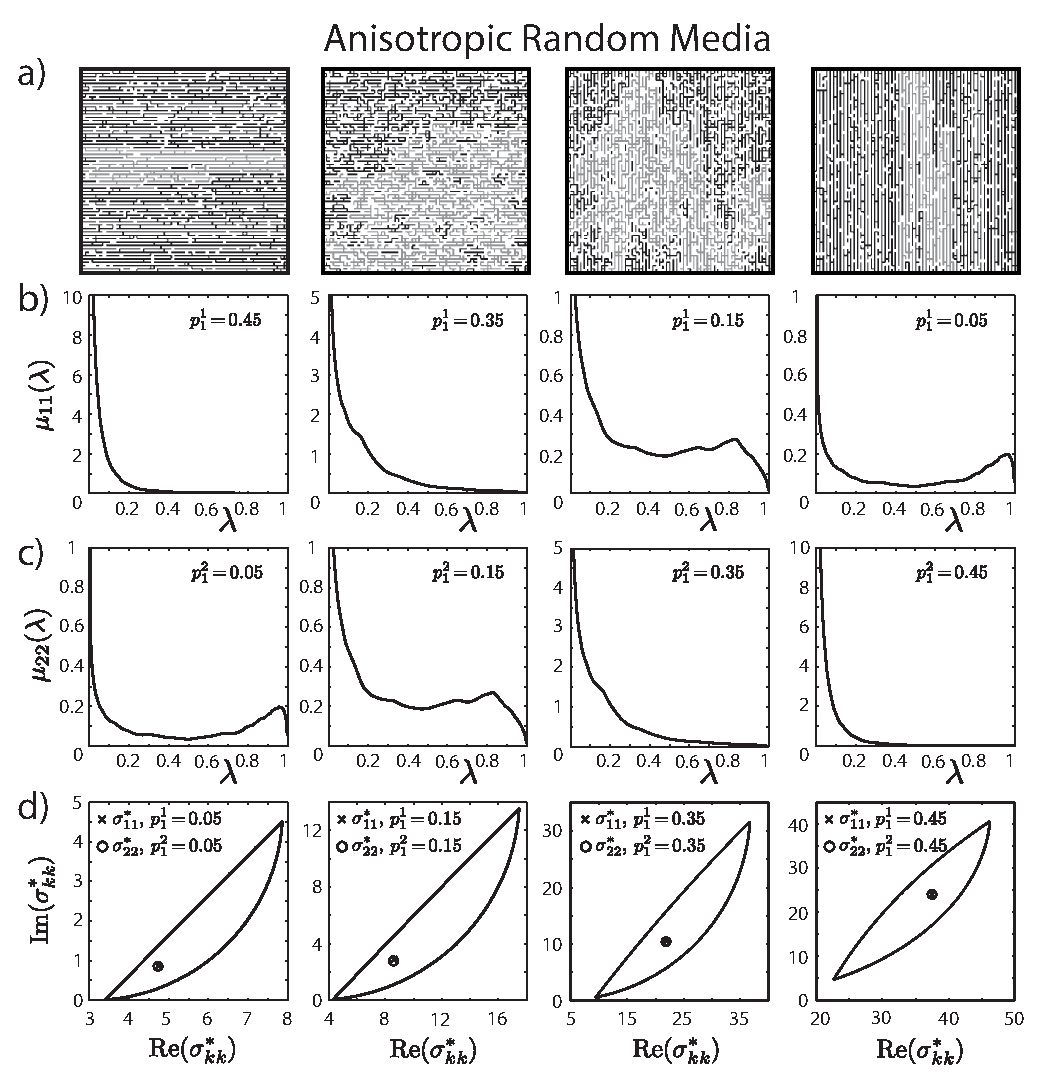
\includegraphics[scale=0.74]{Anisotropic_RRN_p=0_5.eps}} 
\caption{Spectral measures and effective complex conductivities for
  anisotropic random media. Statistical realizations of the 2D square
  bond lattice for $p_1=0.5$ and various values of $p_1^k$, $k=1,2$,
  are displayed in (a). The type-one bonds are colored black, while
  the largest connected cluster of type-one bonds is colored grey. The
  corresponding spectral functions $\mu_{11}(\lambda)$ and $\mu_{22}(\lambda)$ are
  displayed below in (b) and (c), respectively. The effective complex
  conductivities $\sigma^*_{11}$ and $\sigma^*_{22}$ are displayed in (d) for
  $p_1^1=p_1^2$, along with the associated first-order bounds. The
  computed spectral functions have been rescaled so that the area
  under the graph is the measure mass $\mu^0_{kk}=d\,p_1^k$.   
        }
\label{fig:Anisotropic_Spectral_Measures}
\end{figure}
%




%
\begin{figure}[t]
  \centerline{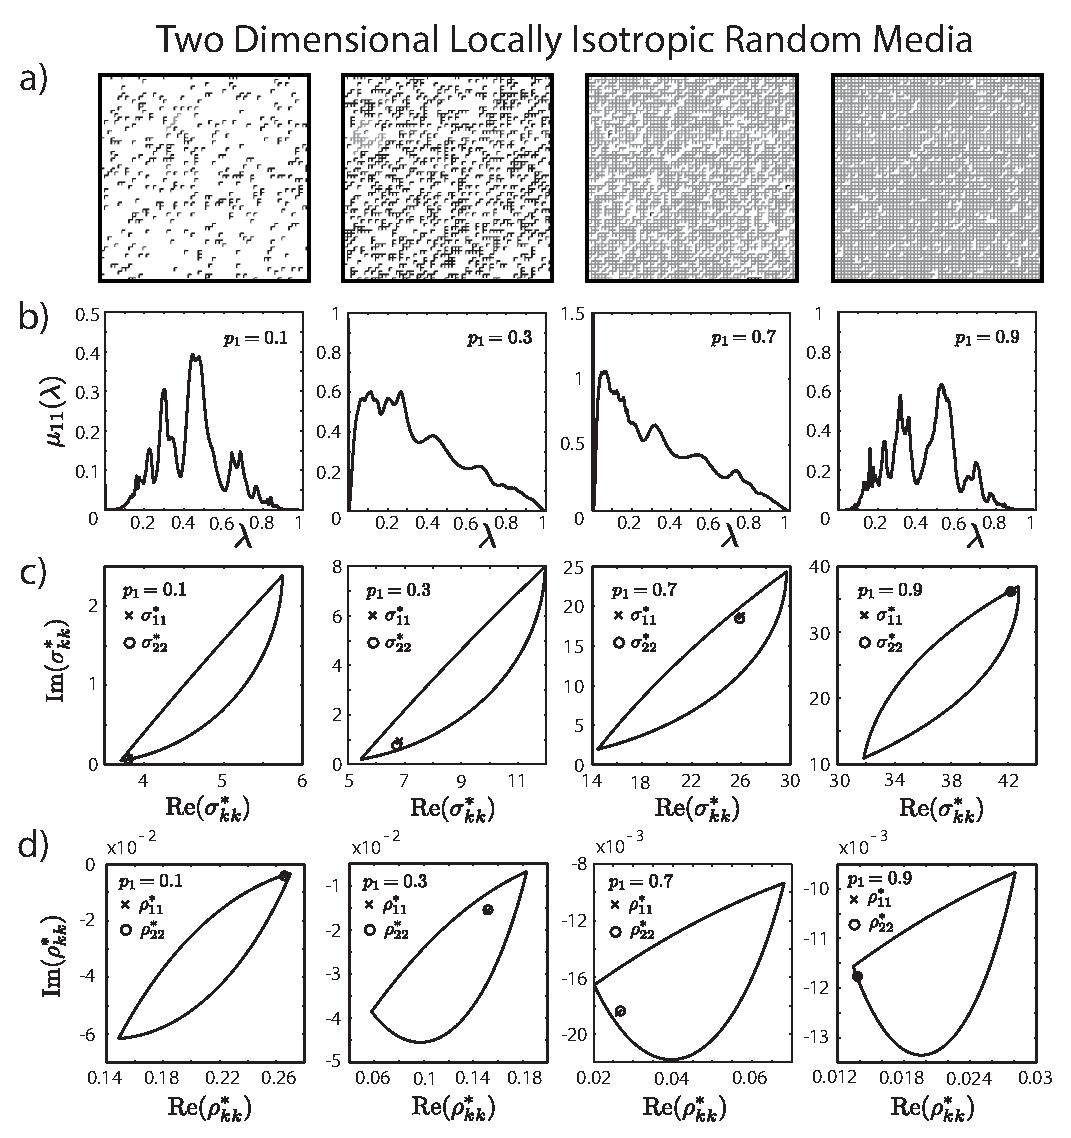
\includegraphics[scale=0.75]{A_Locally_Isotropic_RRN_11.eps}}
\caption{Spectral measures and effective complex conductivities for
  locally isotropic random media. Realizations of the two-dimensional
  lattice model are displayed in (a). The type-one bonds are colored
  black, while the largest connected cluster of type-one bonds is
  colored grey. The corresponding spectral function $\mu_{11}(\lambda)$ is
  displayed in (b) and the effective complex conductivity is displayed
  $\sigma^*_{11}$ in (c), along with the corresponding isotropic
  bounds. The computed spectral functions have been rescaled so that
  the area under the graph is the measure mass $\mu^0_{11}=p_1$.  
        } 
\label{fig:LocIsotropic_RRN_11}
\end{figure}
%


As the system size $L$ increases, the size $N=d\,L^d$ of the matrix
$M_1$, for example, also increases and its eigenvalues become
increasingly dense in the spectral interval $[0,1]$. For a large
enough fixed system, or for a random system averaged over many
statistical realizations, a high resolution histogram representation
of the spectral measure $\mu_{11}$, called the \emph{spectral function}
$\mu_{11}(\lambda)$, begins to resemble a smooth curve, as shown in Figure
\ref{fig:Anisotropic_Spectral_Measures}.






In Figure \ref{fig:Anisotropic_Spectral_Measures}(a) statistical
realizations of the anisotropic 2D bond lattice are displayed for
$L=60$ and a volume (number) fraction $p_1=0.5$ of type-one bonds,
with various values of $p_1^k$, $k=1,2$, the volume fraction of
type-one bonds in the positive $k^{\text{th}}$ direction. In Figure
\ref{fig:Anisotropic_Spectral_Measures}(b) and (c), we display the
behavior of the spectral functions $\mu_{11}(\lambda)$ and $\mu_{22}(\lambda)$,
respectively, as $p_1^k$ varies. In Figure
\ref{fig:Anisotropic_Spectral_Measures}(d) the computed values of the
effective complex conductivities $\sigma^*_{11}$ and $\sigma^*_{22}$ are   
displayed, along with the first order bounds of equation
\eqref{eq:0th_order_Bounds}, which depend only on the mass
$\mu^0_{kk}=d\,p_1^k$ of the measure $\mu_{kk}$ and the value of the contrast parameter
$s=1/(1-\sigma_1/\sigma_2)$. The values of the component conductivities $\sigma_1$
and $\sigma_2$ are taken to be that of the brine and pure ice phase,
respectively, for a sample of sea ice measured at a frequency of
4.75GHz \cite{Backstrom:2007:Book}, $\sigma_1=51.0741+\I\,45.1602$ and 
$\sigma_2=3.07+\I\,0.0019$, yielding
$s\approx-0.034+\I\,0.032$. Consistent with the symmetries of
the model, these spectral functions and effective complex
conductivities satisfy $\mu_{11}(\lambda)=\mu_{22}(\lambda)$ and $\sigma^*_{11}=\sigma^*_{22}$
for $p_1^1=p_1^2$. 



%
%
\begin{figure}[t]
  \centerline{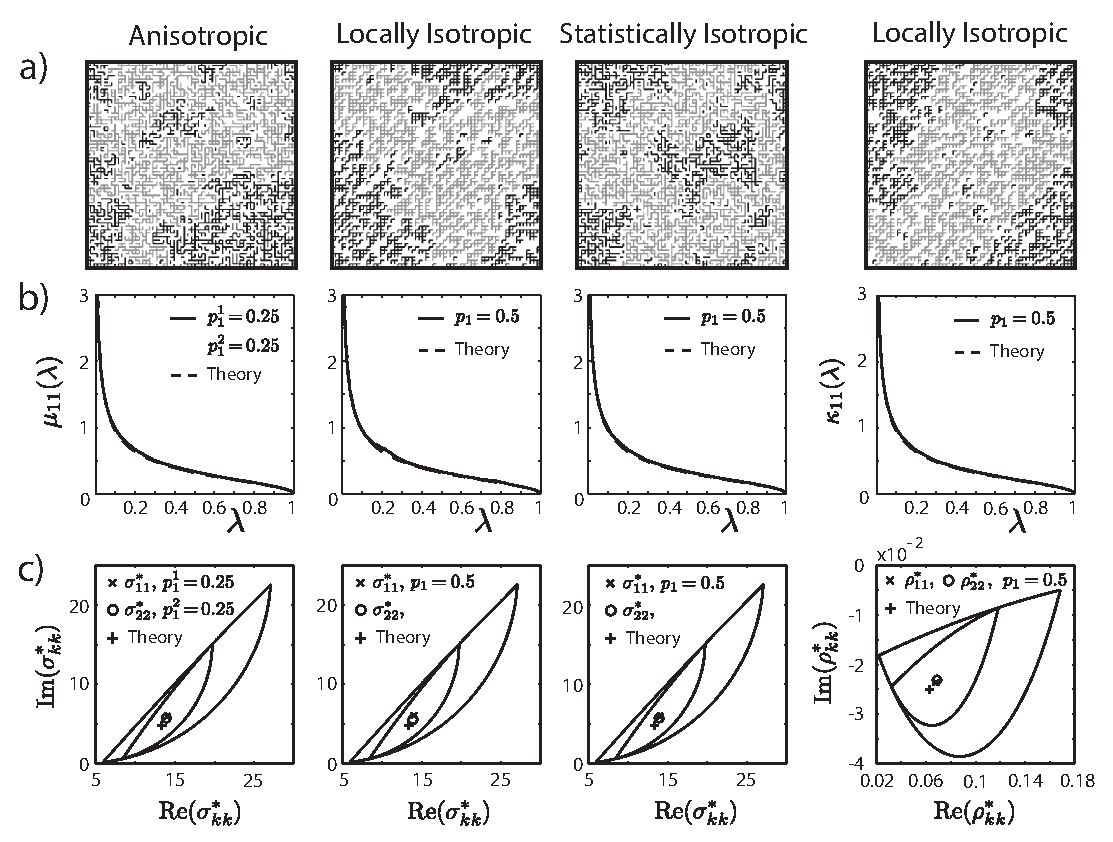
\includegraphics[scale=0.69]{A_Duality_RRN_11.eps}}
\caption{Statistically self-dual random media. Realizations of various 
  two-dimensional lattice models are displayed in (a). The type-one
  bonds are colored black, while the largest connected cluster of
  type-one bonds is colored grey. The corresponding spectral function
  $\mu_{11}(\lambda)$ or $\kappa_{11}(\lambda)$ is displayed in (b) and the effective
  complex conductivity $\sigma^*_{11}$ or resistivity $\rho^*_{11}$ in (c). In
  (b) the theoretical prediction for self-dual composite
  microstructures is also displayed. In (c) the effective 
  complex conductivity or resistivity is displayed along with the
  theoretical prediction and the first-order and isotropic bounds. The
  computed spectral functions have been rescaled so that the area
  under the graph is the measure mass $\mu^0_{11}=p_1$.                
        }
\label{fig:Duality_RRN_11}
\end{figure}
%




We now consider the locally isotropic and statistically isotropic
composite classes introduced 
in the paragraph following the statement of Theorem
\ref{thm:Discrete_Spectral_Theorem_ACM}. In Figure
\ref{fig:LocIsotropic_RRN_11} we display the behavior of the 
spectral function $\mu_{11}(\lambda)$ and the effective complex conductivity
$\sigma^*_{11}$ as a function of $p_1$, for locally isotropic random media
with $L=60$. In Figure \ref{fig:LocIsotropic_RRN_11}(a), statistical
realizations of the composite are displayed. These
spectral functions exhibit a rich resonance structure. These so called
``geometric'' resonances have been attributed
\cite{Jonckheere_Luck_JPA_1998} to the recurrence of local geometric
structures called ``fractal animals.''  In Figure
\ref{fig:LocIsotropic_RRN_11}(c), the corresponding behavior of
$\sigma^*_{11}$ and $\sigma^*_{22}$ is displayed along with the isotropic bounds
of equation \eqref{eq:Isotropic_Bounds}, for the same values of the
component conductivities as that in Figure
\ref{fig:Anisotropic_Spectral_Measures}(c). Consistent with  
isotropy, the behavior of $\mu_{22}(\lambda)$ is very similar to that of
$\mu_{11}(\lambda)$ in Figure \ref{fig:LocIsotropic_RRN_11}(b), and to
numerical accuracy and finite size effects we have
$\sigma^*_{11}=\sigma^*_{22}$. The spectral functions $\mu_{kk}(\lambda)$, $k=1,2$, in
the case of statistically isotropic random media were computed in
\cite{Murphy:JMP:063506}. They look very similar to that for the
locally isotropic case displayed in Figure
\ref{fig:LocIsotropic_RRN_11}(b). Moreover, the spectral functions
$\kappa_{kk}(\lambda)$, $k=1,2$, underlying the effective resistivity $\rho^*_{kk}$,
for locally and statistically isotropic random media also look quite
similar to that for $\mu_{11}(\lambda)$ in Figure
\ref{fig:LocIsotropic_RRN_11}(b). 



%
\begin{figure}[t]
  \centerline{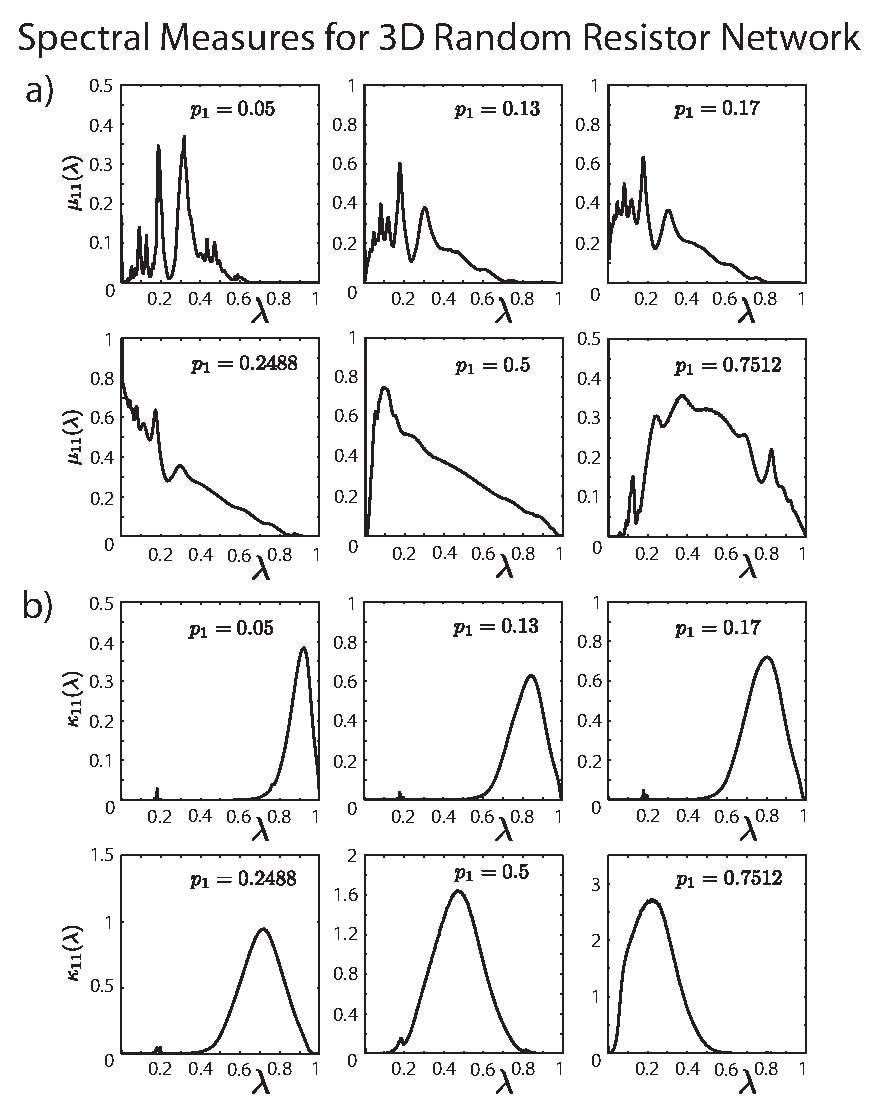
\includegraphics[scale=0.8]{3D_Spectral_Measures_Gamma_GammaCurl.eps}} 
\caption{Spectral measures for 3D locally isotropic random resistor
  network. For various volume fractions $p_1$, the spectral function
  $\mu_{11}(\lambda)$ (a) underlying the effective complex conductivity
  $\sigma^*_{11}$ is displayed with the spectral function $\kappa_{11}(\lambda)$ (b)  
  underlying the effective complex resistivity $\rho^*_{11}$. The
  spectral functions have been rescaled so that the area under the
  graph is the measure mass $\mu^0_{11}=\kappa^0_{11}=p_1$.                
        }
\label{fig:3D_Spectral_Measures}
\end{figure}
%




In the infinite lattice setting, the statistically and locally
isotropic composite microstructures are statistically self-dual for
$d=2$ and $p_1=0.5$ \cite{MILTON:2002:TC}. Note that the class of
anisotropic random media for the special case of $p_1^k=p_1/d$ for all
$k=1,\ldots,d$ is statistically isotropic, and is statistically self-dual
for  $d=2$ and $p_1=0.5$. For such systems, the spectral measures and
effective parameters may be explicitly calculated
\cite{MILTON:2002:TC},
e.g. $\d\mu_{11}(\lambda)=(\sqrt{(1-\lambda)/\lambda}\;)(\d\lambda/\pi)$ and  
$\sigma^*_{11}=\sqrt{\sigma_1\sigma_2}\;$. In Figure \ref{fig:Duality_RRN_11} the 
computed spectral functions and effective parameters are displayed for
such random media in the \emph{finite} lattice setting for $L=60$, and
compared with the theoretical predictions (for the
\emph{infinite} setting). In Figure \ref{fig:Duality_RRN_11}(a), the
bond color scheme for the displayed statistical realizations is the
same as that for Figure \ref{fig:Anisotropic_Spectral_Measures}(a). In
Figure \ref{fig:Duality_RRN_11}(b), the computed spectral functions are 
displayed along with the theoretical prediction. In Figure
\ref{fig:Duality_RRN_11}(c) the computed effective parameters are
displayed with the theoretical prediction, as well as the first-order
and isotropic bounds of equations \eqref{eq:0th_order_Bounds} and
\eqref{eq:Isotropic_Bounds}, respectively, with the same component
conductivities as that in Figure
\ref{fig:Anisotropic_Spectral_Measures}(c). The computed spectral
functions and effective parameters are in excellent agreement with the
theoretical predictions for infinite systems. The error in the computed
values of the effective parameters, relative to the theoretical
prediction, is typically $\lesssim10^{-2}$ for $L=60$ and decreases 
as $L$ increases. 





%
\begin{figure}[t]
  \centerline{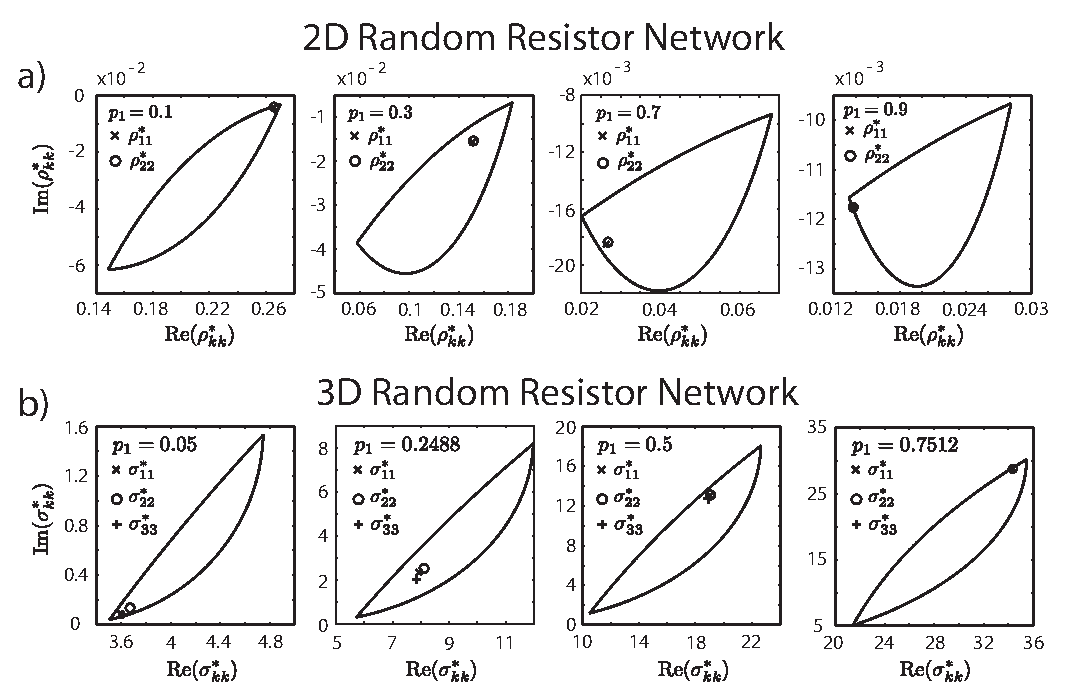
\includegraphics[scale=0.65]{2D_GammaCurl_and_3D_Gamma_Bounds.eps}} 
\caption{Effective complex parameters and isotropic bounds for 2D and
  3D locally isotropic random resistor network (RRN). The behavior of
  the effective complex resistivity $\rho^*_{kk}$, $k=1,2$, for 2D RRN is
  displayed in (a) for various volume fractions $p_1$, along with the
  corresponding isotropic bounds. Similarly, the
  behavior of the effective complex conductivity $\sigma^*_{kk}$,
  $k=1,2,3$, and the corresponding isotropic bounds are displayed for
  3D RRN in (b). 
        }
\label{fig:3D_and_3D_Bounds}
\end{figure}
%








We now discuss the gap behavior of the spectral measures. In the
infinite lattice setting, the isotropic composite 
microstructures discussed in this section are examples of percolation
models, which depend only on the volume fraction $p_1=1-p_2$ of the
constituents, hence $m(h)=m(p_1,h)$, for example. In these lattice
percolation models \cite{Stauffer-92,Torquato:RHM-02}, the bonds are 
open with probability $p_1$, say, and closed with probability
$p_2$. Connected sets of open bonds are called open clusters. The
average cluster size grows as $p_1$ increases, and there is a critical
probability $p_c\,$, $0<p_c<1$, called the \emph{percolation
  threshold}, where an infinite cluster of open bonds first
appears. For the two-dimensional lattice percolation model $p_c=0.5$
and in three-dimensions $p_c\approx0.2488$ 
\cite{Stauffer-92,Torquato:RHM-02}. Now consider transport through the
associated RRN, where the bonds are assigned electrical conductivities
$\sigma_1$ with probability $p_1$ and $\sigma_2$ with probability $p_2$. The
effective conductivity $\sigma^*(p_1,h)$, for example, exhibits two types
of critical behavior as $h=\sigma_1/\sigma_2\to0$. First, when $\sigma_1\to0$ and
$0<\sigma_2<\infty$, $\sigma^*=0$ for $p_1>p_c$ while $\sigma^*>0$ for $p_1<p_c\,$.
% with $\sigma^*(p_1,0)\sim(p-p_c)^t$, as $p\to p_c^+$, where $t$ is the
%conductivity critical exponent 
%, believed to be {\it universal} for lattices depending only on
%dimension. 
Second, when $\sigma_2\to\infty$ and $0<\sigma_1<\infty$, $\sigma^*(p_1,0) \to \infty$ as $p_1\to p_c^+$.
%where $\sigma^*(p,0)\sim(p-p_c)^{-s}$ and $s$ is the superconducting critical
%exponent.


%
\begin{figure}[t]
  \centerline{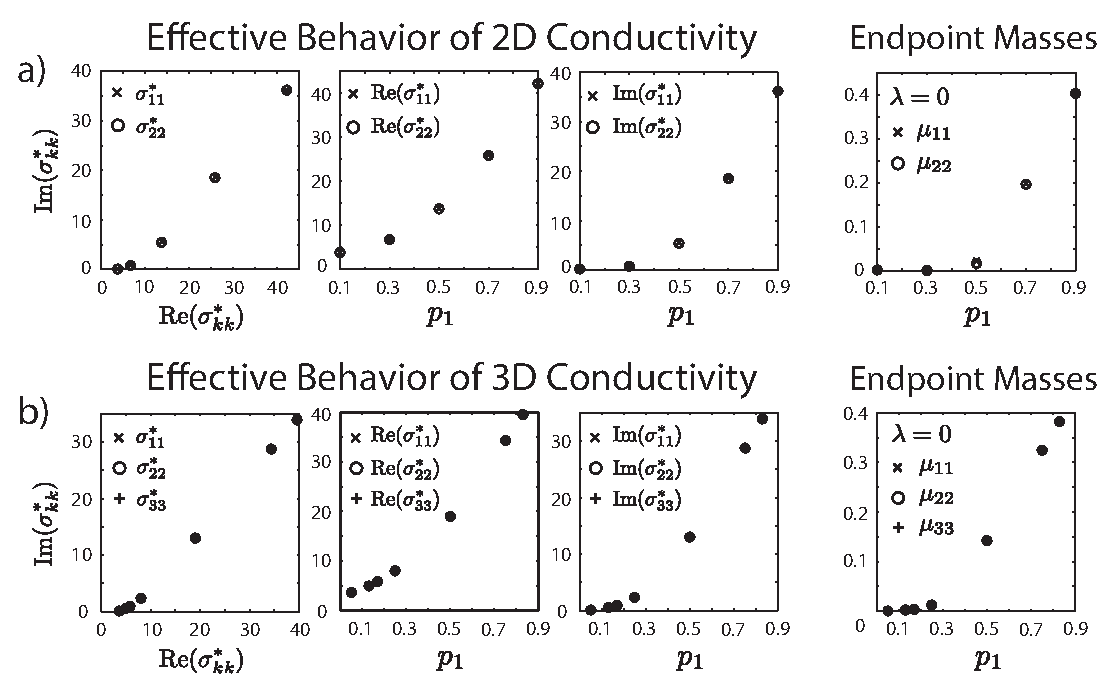
\includegraphics[scale=0.68]{Effective_Parameter_Behavior_4_75GHz.eps}} 
\caption{Behavior of the diagonal components $\sigma^*_{kk}$, $k=1,\ldots,d$, of
  the effective complex conductivity tensor as a function of volume
  fraction $p_1$ for 2D (a) and 3D (b) locally isotropic random
  resistor network. The corresponding mass of the spectral
  measure $\mu_{kk}$ concentrated at $\lambda=0$ is displayed in (c) and (d),
  respectively.   
  %The component conductivities $\sigma_k$ are given by
  %$\sigma_1=51.0741+\I\,45.1602$ and $\sigma_2=3.07+\I\,0.0019$.    
        }
\label{fig:Effective_Parameter_Behavior}
\end{figure}
%







First we consider the two-dimensional lattice percolation model. In
Figures \ref{fig:LocIsotropic_RRN_11}(b) and
\ref{fig:Duality_RRN_11}(b) we see that, as $p_1$ increases from zero 
and the system becomes increasingly connected, gaps in the spectral
function $\mu_{11}(\lambda)$ at the spectral endpoints $\lambda=0,1$ shrink and then
vanish  symmetrically at a value of $p_1=p_c=0.5$. Figure
\ref{fig:Duality_RRN_11}(b) indicates that the vanishing of the gaps
in the spectral function lead to a buildup in the mass of the measure at
$\lambda=0$, while the mass of the measure is approximately zero for $\lambda=1$,
i.e. $\mu_{11}(1)\approx0$.



Now consider the three-dimensional percolation model. In Figure
\ref{fig:3D_Spectral_Measures}(a) and (b) we display 
the behavior of the spectral functions $\mu_{11}(\lambda)$ and $\kappa_{11}(\lambda)$
as $p_1$ varies, for locally isotropic RRN with $L=15$. Like its
2D counterpart, the spectral function $\mu_{11}(\lambda)$ has a rich resonant
structure. Furthermore, as $p_1$ increases from zero and approaches
the percolation threshold $p_c\approx0.2488$, a gap in $\mu_{11}(\lambda)$ about
$\lambda=0$ shrinks and then vanishes, leading to a buildup in the mass of
the measure $\mu_{11}$ at $\lambda=0$ for 
$p_1=p_c$. As $p_1$ increases beyond $p_c$, the mass of $\mu_{11}$ at
$\lambda=0$ continues to grow, while a gap in the spectral function at $\lambda=1$ 
shrinks and then vanishes for $p_1=1-p_c\approx0.7512$, with
$\mu_{11}(1)\approx0$. The associated behavior of the effective complex
conductivity $\sigma^*_{kk}$, $k=1,2,3$, for the 3D 
RRN and its corresponding bounds are displayed in Figure
\ref{fig:3D_and_3D_Bounds}, as well as the effective complex
resistivity $\rho^*_{kk}$, $k=1,2$, for the 2D locally isotropic RRN,
with the same component conductivities as that of Figure
\ref{fig:Anisotropic_Spectral_Measures}(c). Consistent with isotropy,
to numerical accuracy and finite size effects, we have
$\sigma^*_{jj}=\sigma^*_{kk}$ and $\rho^*_{jj}=\rho^*_{kk}$ for all $j,k=1,\ldots,d$. The spectral measures for
\emph{statistically isotropic} 3D RRN  were computed in
\cite{Murphy:JMP:063506} and have a very similar behavior to that for
locally isotropic RRN displayed in Figure
\ref{fig:3D_Spectral_Measures}(a).    



The behavior of the spectral function $\kappa_{11}(\lambda)$ displayed in Figure
\ref{fig:3D_Spectral_Measures}(b) has a similar gap behavior. For a
volume fraction of $p_1=0.001$ (not shown) there is a clear gap in the
spectral function about $\lambda=0$ and $\lambda=1$. The gap near $\lambda=1$ collapses
as $p_1\to p_c$, with $\kappa_{11}(1)\approx0$. As $p_1$ surpasses $p_c$ and
approaches $1-p_c$ the gap in the spectral function near $\lambda=0$
collapses, causing a buildup in the mass of the measure at $\lambda=0$ as
$p_1\to1-p_c$. 





Displayed in Figure \ref{fig:Effective_Parameter_Behavior} is the
behavior of the diagonal components $\sigma^*_{kk}$, $k=1,\ldots,d$, of the
effective complex conductivity tensor as a function of volume fraction
$p_1$, for 2D (a) and 3D (b) locally isotropic RRN. The respective
masses of the measures $\mu_{kk}$, $k=1,\ldots,d$, concentrated at the
spectral endpoint $\lambda=0$ are displayed in (c) and (d).  The component
conductivities are the same as that in Figure
\ref{fig:Anisotropic_Spectral_Measures}(c). It can be seen in Figure
\ref{fig:Effective_Parameter_Behavior} (c) and (d) that for $p_1<p_c$
a very small fraction of the measure mass is concentrated at
$\lambda=0$, where $p_c=0.5$ for 2D and $p_c\approx0.2488$ for 3D. While as $p_1$
surpasses $p_c$, a significant amount of the measure mass becomes
concentrated at the spectral endpoint $\lambda=0$. This $\delta$-function
behavior in the measure at $\lambda=0$ leads to significant changes in
$\sigma^*_{kk}$ as the volume fraction $p_1$ surpasses $p_c$, as can be
seen in this figure. The associated mass of $\mu_{kk}$ concentrated at
$\lambda=1$ is $\sim10^{-30}$ for both 2D and 3D. 

%
\begin{figure}[t]
  \centerline{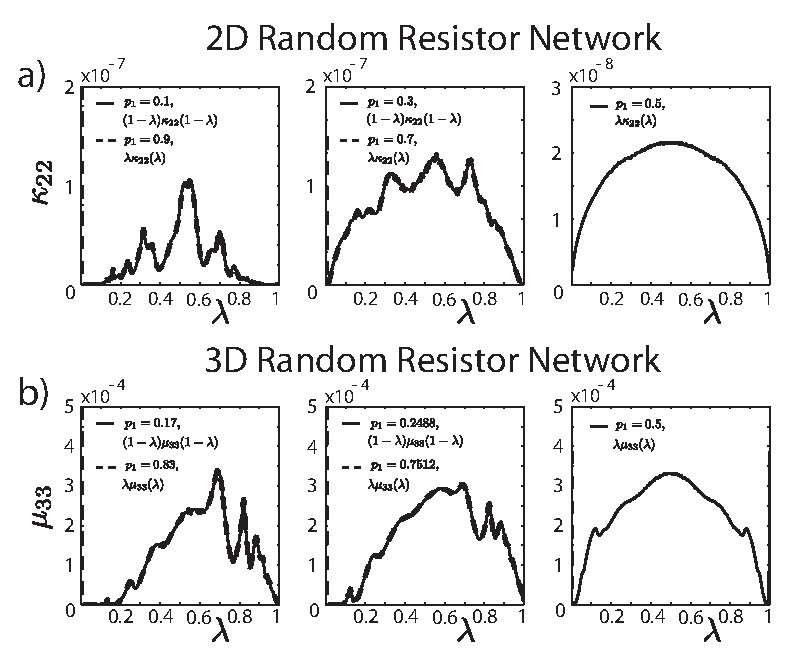
\includegraphics[scale=0.97]{Spectral_Function_Symmetries.eps}} 
\caption{Spectral measure symmetries. Transformations of the computed
  spectral functions for 2D (a) and 3D (b) random resistor network,
  for various values of the volume fraction $p_1$. The computed
  spectral functions have been rescaled to make the area under the
  graph the measure mass.   
        }
\label{fig:Spectral_Function_Symmetries}
\end{figure}
%


This behavior in the spectral measures is consistent with equation
\eqref{eq:Measure_Relations}, which holds for general stationary
random media in the infinite setting \cite{Murphy:JMP:063506}, and
consequently holds for percolation models of such media. This equation
characterizes the percolation transition with the
formation of delta components in the spectral measures at the spectral
endpoints $\lambda=0,1$, \emph{precisely} at $p_1=p_c$ and
$p_1=1-p_c$. Recall that the weights $m_{kk}(0)$ and $w_{kk}(0)$ of
the delta components at $\lambda=0$ and $\lambda=1$ in
\eqref{eq:Measure_Relations}, for example, have the following
behavior. When $\sigma_1=0$ $(h=0$), the function
$m_{kk}(0)=m_{kk}(p_1,0)$, $k=1,\ldots,d$, increases from zero as 
$p_1$ surpasses $p_c$ $(p_1\to p_c^+)$. Similarly, when $\sigma_2=0$
$(z=0)$, the function 
$w_{kk}(0)=w_{kk}(p_2,0)$ increases from zero as $p_1$ surpasses
$1-p_c$ $(p_1\to1-p_c^-)$. For conductor/insulator or
conductor/superconductor systems, this behavior in the spectral
endpoints of the measures lead to critical behavior in the effective
conductivity \cite{Murphy:JMP:063506,Golden:JMP-5627}. 




Equation \eqref{eq:Measure_Relations} also provides a relationship
between the measures $\mu_{jk}$ and $\alpha_{jk}$, and the measures $\eta_{jk}$ and
$\kappa_{jk}$. In Figure \ref{fig:Spectral_Function_Symmetries} we
demonstrate that this relationship between the spectral measures
persists in the finite lattice setting. Displayed in Figure
\ref{fig:Spectral_Function_Symmetries}(a) are graphs of 
transformations of the spectral function $\kappa_{22}(\lambda)$. In particular,
the graph of the function $(1-\lambda)\kappa_{22}(1-\lambda)$ is displayed for
volume fractions $p_1=0.1$, 0.3, and 0.5, along with $\lambda\kappa_{22}(\lambda)$ for
a volume fraction of $1-p_1$. Similarly, in Figure
\ref{fig:Spectral_Function_Symmetries}(b) the graphs of
$(1-\lambda)\mu_{33}(1-\lambda)$ and $\lambda\mu_{33}(\lambda)$ are displayed for various values
of $p_1$ and $1-p_1$, respectively. The graphs of the 
transformed spectral functions are virtually identical except for a
``delta function'' at $\lambda=0$, in excellent agreement with equation
\eqref{eq:Measure_Relations}, which holds for infinite systems.








\section{Conclusion}
%
In Sections \ref{sec:Continuum_Setting} and
\ref{sec:Infinite_Lattice_Setting} we reviewed and extended the ACM for
representing transport in composites, for the \emph{infinite}
continuum and lattice settings. This method provides the Stieltjes
integral representations displayed in \eqref{eq:Stieltjes_F} for the
effective parameters of two-phase random media, involving spectral
measures associated with the self-adjoint random operators
$M_i=\chi_i\Gamma\chi_i$ and $K_i=\chi_i\Upsilon\chi_i$. Here, $\chi_i$ is the characteristic function
for material phase $i=1,2$ and the operators
$\Gamma=\vec{\nabla}(\Delta^{-1})\vec{\nabla}\cdot$ and $\Upsilon=-\vec{\nabla}\times(\bDelta^{-1})\vec{\nabla}\times$
act as projectors onto curl-free and divergence-free fields,
respectively. 






In Section \ref{sec:Finite_Lattice_Setting} we developed the ACM for
the \emph{finite} lattice setting. We also provided a projection
method for numerically efficient, rigorous computation of spectral
measures and effective parameters for such composite media. This
projection method is summarized by equations
\eqref{eq:Spec_Decomp_chi_Gamma_chi} and
\eqref{eq:measure_equivalence} of Theorem
\ref{thm:Discrete_Spectral_Theorem_ACM}, which is a key theoretical
contribution of this work. In this finite lattice case, the operators
$\chi_i$, $\Gamma$, and $\Upsilon$ are represented by real-symmetric projection
matrices, and the spectral measures of the associated real-symmetric
random matrices $M_i$ and $K_i$ are given explicitly in terms of their
eigenvalues and eigenvectors, as displayed in equation
\eqref{eq:Stieltjes_F_Discrete} of Theorem
\ref{thm:Discrete_Spectral_Theorem_ACM}. 



In the paragraph following the statement of Theorem
\ref{thm:Discrete_Spectral_Theorem_ACM}, we introduced three 
families of locally isotropic, statistically isotropic, and
anisotropic random media on finite bond lattices. In Section
\ref{sec:Numerical_Results} we employed the projection method to
compute the spectral measures and effective parameters associated with
these families of random media. To our knowledge, this is the first
time that the spectral measures $\eta_{jk}$ and $\kappa_{jk}$ underlying the
effective complex resistivity $\rho^*_{jk}$ have been computed for such
composite microstructures. These computations not only demonstrate
several important properties of the spectral measures and the
associated effective parameters, but they also serve as a consistency
check to the theory developed here.



The computed spectral functions and effective complex parameters for
anisotropic random media, displayed in Figure
\ref{fig:Anisotropic_Spectral_Measures},  are consistent with the
symmetries of the model. Consistent with general theory
\cite{MILTON:2002:TC}, our computations of the effective parameters
for isotropic random media 
satisfy $\sigma^*_{kk}=1/\rho^*_{kk}$, $k=1,\ldots,d$ (to numerical accuracy and
statistical truncation). Moreover, the computed spectral functions and
effective parameters are consistent with isotropy and satisfy
$\mu_{jj}(\lambda)=\mu_{kk}(\lambda)$ and $\sigma^*_{jj}=\sigma^*_{kk}$, for example, for all
$j,k=1,\ldots,d$ (to numerical accuracy, finite size effects, and
statistical truncation). Figure
\ref{fig:Duality_RRN_11} demonstrates that the projection method
accurately calculates the spectral measures and 
effective parameters for statistically self-dual composite
microstructures. Furthermore, Figure
\ref{fig:Spectral_Function_Symmetries} shows that the computed 
spectral measures are in excellent agreement with equation
\eqref{eq:Measure_Relations}, which holds for general stationary
two-phase random media \cite{Murphy:JMP:063506}. 



The self-consistent mathematical framework developed here helps lay
the groundwork for studies in the effective transport properties of a
broad range of important composites, such as electrorheological
fluids \cite{Murphy_Thermo_Stat_Mech}, multiscale sea ice structures
\cite{Murphy_Multiscale_Sea_Ice}, and bone
\cite{Golden:JBM:337}. Remarkably, the ACM  has also been
adapted to provide Stieltjes integral representations for 
effective parameters underlying a wide variety of transport processes,
such as: the effective diffusivity for steady
\cite{McLaughlin:SIAM_JAM:780,Avellaneda:CMP-339,Murphy_Advective_Diffusion}
and time-dependent \cite{Avellaneda:PRE:3249} turbulent flows, the
effective complex permittivity for uniaxial polycrystalline media 
\cite{Barabash:JPCM:10323,Gully_Golden_Polycrystalline}, and the
effective elastic moduli of two-phase elastic composites
\cite{Ou:2012:411,Ou:MMAS:655}. The Golden-Papanicolaou formulation of
the ACM has been pivotal in the development of these mathematical
frameworks, and in the understanding of these important transport
processes. 


%\newpage

% redefine the command that creates the equation no.
  \setcounter{equation}{1}  % reset equation counter
  \setcounter{section}{0}  % reset section counter
  \renewcommand{\theequation}{A-\arabic{equation}} 
\renewcommand{\thesection}{A-\arabic{section}}
\section{Appendix: The Spectral Theorem} 
\label{sec:The_Spectral_Theorem}
%
In this appendix we review the spectral theorem as it pertains to the
ACM, for both the bounded linear self-adjoint operator setting
\cite{Reed-1980,Stone:64} and the real-symmetric matrix setting
\cite{Kreyszig:JWS-1989,Halmos-1958,Stakgold:BVP:2000}, leading to equations
\eqref{eq:Stieltjes_F} and \eqref{eq:Stieltjes_F_Discrete}, 
respectively. In Section \ref{sec:The_Spectral_Theorem_Continuum} we
review the spectral theorem associated with the bounded linear
self-adjoint operators $M_i=\chi_i\Gamma\chi_i$ and $K_i=\chi_i\Upsilon\chi_i$, $i=1,2$, which
arise naturally in the ACM for the continuum and infinite lattice
settings discussed in Sections \ref{sec:Continuum_Setting} and
\ref{sec:Infinite_Lattice_Setting}, respectively.  In Section 
\ref{sec:The_Spectral_Theorem_Finite_Lattice} we discuss the spectral 
theorem for the finite lattice setting discussed in Section
\ref{sec:Finite_Lattice_Setting}, where the operators $M_i$ and $K_i$
are represented by real-symmetric random matrices. In each case we
obtain Stieltjes integral representations for $\bsig^*$ and $\brho^*$,
as displayed in equations \eqref{eq:Stieltjes_F} and
\eqref{eq:Stieltjes_F_Discrete}, involving matrix valued spectral
measures. 
%
\subsection{Continuum  and Infinite Lattice Settings}
\label{sec:The_Spectral_Theorem_Continuum} 
%
In Section \ref{sec:Continuum_Setting} we introduced the Herglotz 
functions $m_{jk}(h)$, $w_{jk}(z)$, $\tilde{m}_{jk}(h)$, and
$\tilde{w}_{jk}(z)$, and the respective measures $\mu_{jk}$, $\alpha_{jk}$,
$\eta_{ij}$, and $\kappa_{jk}$ underlying their Stieltjes integral
representations in \eqref{eq:Stieltjes_F}. Due to the many symmetries
between these functions and measures, we focused on $m_{jk}(h)$ and
$\mu_{jk}$, as the discussions involving the other functions and
measures follow by direct analogy. For simplicity, we will continue
this approach here.  



In the paragraph proceeding that which involves equation
\eqref{eq:Stieltjes_F}, we argued that on the Hilbert space
$\mathscr{H}_\times$ with weight $\chi_1$ in the inner-product,
$\langle\cdot,\cdot\rangle_1=\langle\chi_1\,\cdot,\cdot\rangle$, the composition $\Gamma\chi_1$ of projection operators
is a bounded linear self-adjoint operator with spectrum contained in
the interval $[0,1]$. The spectral theorem for bounded linear
operators in Hilbert space \cite{Stone:64} states that there is a
one-to-one correspondence between the operator $\Gamma\chi_1$ and a family of
self-adjoint projection operators $Q(\lambda)$ parameterized by $\lambda\in[0,1]$
--- the resolution of the identity --- that satisfies
$\lim_{\lambda\to0}Q(\lambda)=0$ and $\lim_{\lambda\to1}Q(\lambda)=I$. Moreover,
COVER THE GENERAL STATEMENT OF THE THEOREM INCLUDING THE DOMAIN OF THE OPERATOR
INVOLVING GENERAL ELEMENTS OF THE HILBERT SPACE $\xi$ and $\zeta$
% 
\begin{align}\label{eq:Spectral_Theorem}  
  \langle f(M_1)\,\vec{e}_j\cdot\vec{e}_k\rangle_1= \int_0^1f(\lambda)\d\mu_{jk}(\lambda), \quad
  \mu_{jk}(\lambda)=\langle Q(\lambda)\vec{e}_j,\vec{e}_k\rangle_1
\end{align}
%
for all complex valued functions $f\in L^2(\mu_{jk})$ \cite{Stone:64}. Here
$0$ and $I$ are the null and identity operators on $\mathbb{R}^d$,
respectively and $\d\mu_{jk}(\lambda)=\d\langle Q(\lambda)\,\vec{e}_j\cdot\vec{e}_k\rangle_1$,
$j,k=1,\ldots,d$, are the components of the matrix valued \emph{spectral
  measure} $\d\bmu(\lambda)$ in the $(\vec{e}_j,\vec{e}_k)$ state
\cite{Golden:CMP-473,Reed-1980,Stone:64}. As the spectrum of the 
operator $M_1$ is contained in the interval $[0,1]$, the support
$\Sigma_{jk}$ of the measure $\mu_{jk}$ satisfies $\Sigma_{jk}\subseteq[0,1]$
\cite{Reed-1980}. Setting $f(\lambda)=(s-\lambda)^{-1}$ in
\eqref{eq:Spectral_Theorem} yields the the integral formula for 
$F_{jk}(s)$ and $\sigma_{jk}^*=\sigma_2m_{jk}(h)$ in equation \eqref{eq:Stieltjes_F}.




\subsection{Finite Lattice Setting}
\label{sec:The_Spectral_Theorem_Finite_Lattice}
%
In this section we derive discrete versions of the integral
representation given in equation  \eqref{eq:Spectral_Theorem}. This
leads to the discrete integral representation for the effective
conductivity tensor $\bsig^*$ displayed in equation
\eqref{eq:Stieltjes_F_Discrete}. Toward this goal, we defined in
Section \ref{sec:Finite_Lattice_Setting} a bijective mapping
$\Theta:\mathbb{Z}_L^d\to\mathbb{N}_L$ from the finite $d$-dimensional bond
lattice $\mathbb{Z}_L^d$ defined in \eqref{eq:ZLd} onto the one
dimensional set $\mathbb{N}_L$ defined in equation
\eqref{eq:Bijection_Z_N}. Moreover we showed that, under the mapping
$\Theta$, the random operator $M_1=\chi_1\Gamma\chi_1$ can be represented as a
\emph{real-symmetric} random matrix of size $N\times N$, where $N=d\,L^d$,
$d$ is the dimension of the system, and $L$ is the lattice size
\cite{Golden:JBM:337,Murphy:JMP:063506}. More specifically, $\Gamma$
is a \emph{non-random} real-symmetric projection matrix ($\Gamma^2=\Gamma$) and
$\chi_1$ is a \emph{random} diagonal projection matrix with zeros and
ones along the main diagonal, and has the block diagonal form
displayed in equation \eqref{eq:block_diag_chi}. Since $M_1(\omega)$ is a
composition of projection matrices, it is a positive definite matrix,
$M_1(\omega)\vec{\xi}\cdot\vec{\xi}=(\Gamma\chi_1(\omega)\vec{\xi})\cdot(\Gamma\chi_1(\omega)\vec{\xi})\geq0$ for every
$\omega\in\Omega$ and $\vec{\xi}\in\mathbb{R}^N$, and consequently has spectra
$\Sigma^\lambda(\omega)\subseteq[0,1]$ \cite{Horn_Johnson-1990,Demmel:1997}.   






It is well known \cite{Horn_Johnson-1990,Keener-2000} that the
eigenvectors $\vec{u}_i(\omega)$, $i=1,\ldots,N$, of the symmetric matrix
$M_1(\omega)$ form an orthonormal 
basis for $\mathbb{R}^N$, for each $\omega\in\Omega$, i.e., 
$\vec{u}_j^{\,T}\vec{u}_k=\delta_{jk}$  and for every
$\vec{\xi}\in\mathbb{R}^N$ we have
$\vec{\xi}=\sum_{i=1}^N(\vec{u}_i^{\,T}\vec{\xi}\;)\vec{u}_i  
=\left(\sum_{i=1}^N\vec{u}_i\vec{u}_i^{\,T}\right)\vec{\xi}\,$. Consequently,       
%
\begin{align}\label{eq:Matrix_Rep_Spec_Theorem}
  \sum_{i=1}^NQ_i(\omega)=I, \quad
  Q_i(\omega)=\vec{u}_i(\omega)\vec{u}_i^{\,T}(\omega),  \quad
  \forall \     \omega\in\Omega,
\end{align}
%
where $I$ is the identity operator on $\mathbb{R}^N$ and the matrix
$Q_i$ is the orthogonal projector ($Q_iQ_j=Q_i\delta_{ij}$) onto the
eigenspace spanned by $\vec{u}_i$, which is associated with the
\emph{real} eigenvalue $\lambda_i(\omega)\in\Sigma^\lambda(\omega)$. 


Since $M_1\vec{u}_i=\lambda_i\vec{u}_i$, for each $i=1,\ldots,N$, equation
\eqref{eq:Matrix_Rep_Spec_Theorem} implies that we also have
$M_1Q_i=\lambda_iQ_i$ which, in turn, implies that the matrix  $M_1$ has the
spectral decomposition $M_1=\sum_{i=1}^N\lambda_iQ_i$. By the orthogonality of
the projection matrices $Q_i$ and by induction we have
$M_1^n=\sum_{i=1}^N\lambda_i^nQ_i$ for all $n\in\mathbb{N}$, which implies that
$f(M_1)=\sum_{i=1}^Nf(\lambda_i)Q_i$ for any polynomial
$f:\mathbb{C}\mapsto\mathbb{C}$.  This formula is a discrete version of the
first formula in equation \eqref{eq:Spectral_Theorem} for polynomial
$f(\lambda)$, and leads to a discrete version of the functional
representation of  $f(M_1)$ in \eqref{eq:Spectral_Theorem} involving a
matrix valued spectral measure $\d\bmu(\lambda)$ with components $\d\mu_{jk}(\lambda)$
%
\begin{align}\label{eq:Discrete_Spectral_Theorem}
%f(M_1)=\sum_{i=1}^Nf(\lambda_i)Q_i, \quad
  \langle f(M_1)\hat{e}_j\cdot\hat{e}_k\rangle= \int_0^1f(\lambda)\d\mu_{jk}(\lambda), \quad
  \d\mu_{jk}(\lambda)=\sum_{i=1}^N\langle\delta_{\lambda_i}(\d\lambda)Q_i\,\hat{e}_j\cdot\hat{e}_k\rangle.
\end{align}
%
Here, $Q(\lambda)=\sum_{i:\lambda_i<\lambda}\delta_{\lambda_i}(\d\lambda)Q_i$ is a discrete version of the
projection valued measure introduced in equation
\eqref{eq:Spectral_Theorem}, $\delta_{\lambda_i}(\d\lambda)$ is the Dirac measure
concentrated at $\lambda_i$, the orthonormal vectors
$\hat{e}_i=\Theta(\vec{e}_i)/L^{d/2}$, for $i=1,\ldots,d$, represent the standard
basis vectors on $\mathbb{N}_L$, and $\langle\cdot\rangle$ denotes ensemble
average over $\Omega$. The spectral end points $\lambda_{jk}^0$ and $\lambda_{jk}^1$ of the
support $\Sigma_{jk}\subseteq[\lambda_{jk}^0,\lambda_{jk}^1]\subseteq[0,1]$ of the measure $\mu_{jk}$ in
\eqref{eq:Discrete_Spectral_Theorem} are given by
$\lambda_{jk}^0=\inf A_{jk}$ and $\lambda_{jk}^1=\sup A_{jk}$, where
%
\begin{align}
 % \lambda_{jk}^0=\inf A_{jk}, \quad \lambda_{jk}^1=\sup A_{jk}, \quad
  A_{jk}= \cup_{\omega\in\Omega}\{\lambda_i(\omega)\in\Sigma^\lambda(\omega), \   i=1,\ldots,N \ | \ Q_i(\omega)\hat{e}_j\cdot\hat{e}_k\neq0\}
  % \lambda_{jk}^0&=\inf \cup_{\omega\in\Omega}\{\lambda_i(\omega)\in\Sigma^\lambda(\omega), \
%   i=1,\ldots,N \ | \ Q_i(\omega)\hat{e}_j\cdot\hat{e}_k\neq0\},\\
%   \lambda_{jk}^1&=\sup \cup_{\omega\in\Omega}\{\lambda_i(\omega)\in\Sigma^\lambda(\omega), \
%   i=1,\ldots,N \ | \ Q_i(\omega)\hat{e}_j\cdot\hat{e}_k\neq0\},\notag
\end{align}
%
and $\Sigma^\lambda_1(\omega)\subseteq[0,1]$ is the support of the eigenvalues of the matrix
$M_1(\omega)$ for $\omega\in\Omega$. 



We now show that equation \eqref{eq:Discrete_Spectral_Theorem} also
holds for the function $f(\lambda)=(s-\lambda)^{-1}$ when
$s\in[0,1]\backslash\mathbb{C}$. For each $\omega\in\Omega$, let $U(\omega)$ denote the matrix
with columns consisting of the orthonormal eigenvectors $\vec{u}_i(\omega)$
of $M_1(\omega)$ and let $\Lambda(\omega)=\text{diag}(\lambda_1(\omega),\ldots,\lambda_N(\omega))$ denote the
diagonal matrix of the corresponding eigenvalues $\lambda_i(\omega)$, $i=1,\ldots,N$,
so that $M_1=U\Lambda U^T$ \cite{Horn_Johnson-1990}. By the orthogonality,
$U^TU=UU^T=I$, of the matrix $U$ \cite{Horn_Johnson-1990} we have   
%
\begin{align}\label{eq:Discrete_Stieltjes_F_Derivation}
     \langle f(M_1)\hat{e}_j\cdot\hat{e}_k\rangle
        &=\langle(sI-U\Lambda U^T)^{-1}\hat{e}_j\cdot\hat{e}_k\rangle
        = \langle U(sI-\Lambda)^{-1}U^T\hat{e}_j\cdot\hat{e}_k\rangle\\
        &=\langle(sI-\Lambda)^{-1}U^T\hat{e}_j\cdot U^T\hat{e}_k\rangle
       % =\sum_{i=1}^N\left\langle
       %      \frac{(\vec{u}_i^{\,T}\hat{e}_j)(\vec{u}_i^{\,T}\hat{e}_k)}{s-\lambda_i}
       %        \right\rangle
        =\sum_{i=1}^N\left\langle
          \frac{Q_i\hat{e}_j}{s-\lambda_i}\cdot\hat{e}_k
          \right\rangle.               
%        m_{ij}(i)=\langle Q_i\hat{e}_i,\hat{e}_j\rangle
%                =\langle(\vec{u}_i^{\,T}\hat{e}_i)(\vec{u}_i^{\,T}\hat{e}_j)\rangle,
        \notag
\end{align}
%
Equation \eqref{eq:Discrete_Stieltjes_F_Derivation} is equivalent to equation
\eqref{eq:Discrete_Spectral_Theorem} when the function
$f(\lambda)=(s-\lambda)^{-1}$, $s\in\mathbb{C}\backslash[0,1]$.





\medskip

{\bf Acknowledgements.}
We gratefully acknowledge support from the Division of Mathematical
Sciences and the Office of Polar Programs at the U.S. 
National Science Foundation (NSF) through Grants
DMS-1009704, ARC-0934721, and DMS-0940249. We are also grateful for 
support from the Office of Naval Research (ONR) through
Grants N00014-13-10291 and N00014-12-10861. Finally, we would like to 
thank the NSF Math Climate Research Network (MCRN) for their support
of this work. 


\medskip

\bibliographystyle{siam}
\bibliography{murphy}
\end{document}

% LocalWords:  CMS RM al holomorphy nite DEFORMABLE Nonsimple Varadhan JPA Stat
% LocalWords:  Mech iY jY dL jk eps def rep Ef Jf jL Det ccc diag chi iid Cond
% LocalWords:  Decomp Perm Eigenspace ui Ri Es PtI ELENA mh Fs Hashin Shtrikman
% LocalWords:  extremized kk eigenspace Nf ij GRAEME'S Acknowledgement murphy
